% Options for packages loaded elsewhere
\PassOptionsToPackage{unicode}{hyperref}
\PassOptionsToPackage{hyphens}{url}
%
\documentclass[
]{article}
\usepackage{amsmath,amssymb}
\usepackage{iftex}
\ifPDFTeX
  \usepackage[T1]{fontenc}
  \usepackage[utf8]{inputenc}
  \usepackage{textcomp} % provide euro and other symbols
\else % if luatex or xetex
  \usepackage{unicode-math} % this also loads fontspec
  \defaultfontfeatures{Scale=MatchLowercase}
  \defaultfontfeatures[\rmfamily]{Ligatures=TeX,Scale=1}
\fi
\usepackage{lmodern}
\ifPDFTeX\else
  % xetex/luatex font selection
\fi
% Use upquote if available, for straight quotes in verbatim environments
\IfFileExists{upquote.sty}{\usepackage{upquote}}{}
\IfFileExists{microtype.sty}{% use microtype if available
  \usepackage[]{microtype}
  \UseMicrotypeSet[protrusion]{basicmath} % disable protrusion for tt fonts
}{}
\makeatletter
\@ifundefined{KOMAClassName}{% if non-KOMA class
  \IfFileExists{parskip.sty}{%
    \usepackage{parskip}
  }{% else
    \setlength{\parindent}{0pt}
    \setlength{\parskip}{6pt plus 2pt minus 1pt}}
}{% if KOMA class
  \KOMAoptions{parskip=half}}
\makeatother
\usepackage{xcolor}
\usepackage[margin=1in]{geometry}
\usepackage{graphicx}
\makeatletter
\def\maxwidth{\ifdim\Gin@nat@width>\linewidth\linewidth\else\Gin@nat@width\fi}
\def\maxheight{\ifdim\Gin@nat@height>\textheight\textheight\else\Gin@nat@height\fi}
\makeatother
% Scale images if necessary, so that they will not overflow the page
% margins by default, and it is still possible to overwrite the defaults
% using explicit options in \includegraphics[width, height, ...]{}
\setkeys{Gin}{width=\maxwidth,height=\maxheight,keepaspectratio}
% Set default figure placement to htbp
\makeatletter
\def\fps@figure{htbp}
\makeatother
\setlength{\emergencystretch}{3em} % prevent overfull lines
\providecommand{\tightlist}{%
  \setlength{\itemsep}{0pt}\setlength{\parskip}{0pt}}
\setcounter{secnumdepth}{5}
\newlength{\cslhangindent}
\setlength{\cslhangindent}{1.5em}
\newlength{\csllabelwidth}
\setlength{\csllabelwidth}{3em}
\newlength{\cslentryspacingunit} % times entry-spacing
\setlength{\cslentryspacingunit}{\parskip}
\newenvironment{CSLReferences}[2] % #1 hanging-ident, #2 entry spacing
 {% don't indent paragraphs
  \setlength{\parindent}{0pt}
  % turn on hanging indent if param 1 is 1
  \ifodd #1
  \let\oldpar\par
  \def\par{\hangindent=\cslhangindent\oldpar}
  \fi
  % set entry spacing
  \setlength{\parskip}{#2\cslentryspacingunit}
 }%
 {}
\usepackage{calc}
\newcommand{\CSLBlock}[1]{#1\hfill\break}
\newcommand{\CSLLeftMargin}[1]{\parbox[t]{\csllabelwidth}{#1}}
\newcommand{\CSLRightInline}[1]{\parbox[t]{\linewidth - \csllabelwidth}{#1}\break}
\newcommand{\CSLIndent}[1]{\hspace{\cslhangindent}#1}
\usepackage{setspace}\doublespacing
\usepackage[fontsize=12pt]{scrextend}
\usepackage[left]{lineno}
\usepackage[labelformat=empty]{caption}
\usepackage{longtable}
\usepackage{booktabs}
\usepackage{booktabs}
\usepackage{longtable}
\usepackage{array}
\usepackage{multirow}
\usepackage{wrapfig}
\usepackage{float}
\usepackage{colortbl}
\usepackage{pdflscape}
\usepackage{tabu}
\usepackage{threeparttable}
\usepackage{threeparttablex}
\usepackage[normalem]{ulem}
\usepackage{makecell}
\usepackage{xcolor}
\ifLuaTeX
  \usepackage{selnolig}  % disable illegal ligatures
\fi
\IfFileExists{bookmark.sty}{\usepackage{bookmark}}{\usepackage{hyperref}}
\IfFileExists{xurl.sty}{\usepackage{xurl}}{} % add URL line breaks if available
\urlstyle{same}
\hypersetup{
  hidelinks,
  pdfcreator={LaTeX via pandoc}}

\author{}
\date{\vspace{-2.5em}}

\begin{document}

\hypertarget{title-page}{%
\section*{Title Page}\label{title-page}}

\textbf{Supplement: Bimodal Inference in Humans and Mice}\\
\strut \\

\textbf{Authors}:

Veith Weilnhammer\(^{1,2}\), Heiner Stuke\(^{1,2}\), Kai
Standvoss\(^{1,3,5}\), Philipp Sterzer\(^{6}\)\\
\strut \\
\textbf{Affiliations}:

\(^{1}\) Department of Psychiatry, Charité-Universitätsmedizin Berlin,
corporate member of Freie Universität Berlin and Humboldt-Universität zu
Berlin, 10117 Berlin, Germany\\
\(^{2}\) Berlin Institute of Health, Charité-Universitätsmedizin Berlin
and Max Delbrück Center, 10178 Berlin, Germany\\
\(^{3}\) Bernstein Center for Computational Neuroscience,
Charité-Universitätsmedizin Berlin, 10117 Berlin, Germany\\
\(^{4}\) Berlin School of Mind and Brain, Humboldt-Universität zu
Berlin, 10099 Berlin, Germany\\
\(^{5}\) Einstein Center for Neurosciences Berlin, 10117 Berlin,
Germany\\
\(^{6}\) Department of Psychiatry (UPK), University of Basel,
Switzerland\\
\strut \\

\textbf{Corresponding Author}:

Veith Weilnhammer, Department of Psychiatry, Charité Campus Mitte,
Charitéplatz 1, 10117 Berlin, phone: 0049 (0)30 450 517 317, email:
\href{mailto:veith.weilnhammer@gmail.com}{\nolinkurl{veith.weilnhammer@gmail.com}}\\

\newpage

\linenumbers

\hypertarget{supplemental-items}{%
\section{Supplemental Items}\label{supplemental-items}}

\hypertarget{internal-mode-processing-is-driven-by-choice-history-as-opposed-to-stimulus-history}{%
\subsection{Internal mode processing is driven by choice history as
opposed to stimulus
history}\label{internal-mode-processing-is-driven-by-choice-history-as-opposed-to-stimulus-history}}

The main manuscript reports the effects of perceptual history, which we
defined as the impact of the choice at the preceding trial on the choice
at the current trial (henceforth \emph{choice history}). \emph{Stimulus
history}, which is defined as the impact of the stimulus presented at
the preceding trial on the choice at the present trial, represents an
alternative approach to this. Here, we compare the effects of choice
history to the effects of stimulus history.

We observed a significant bias toward stimulus history (humans: 49.76\%
± 0.1\% of trials, \(\beta\) = \(1.26\) ± \(0.94\), T(\(373.62\)) =
\(1.34\), p = \(0.18\); mice: 51.11\% ± 0.08\% of trials, T(164) = 13.4,
p = \(\ensuremath{3.86\times 10^{-28}}\)). The bias toward stimulus
history was smaller than the bias toward choice history (humans:
\(\beta\) = \(-3.53\) ± \(0.5\), T(\(66.53\)) = \(-7.01\), p =
\(\ensuremath{1.48\times 10^{-9}}\); mice: T(164) = -17.21, p =
\(\ensuremath{1.43\times 10^{-38}}\)).

The attraction of choices toward both preceding choices and stimuli is
expected, as perception was \emph{stimulus-congruent} on approximately
75\% of trials, causing choices and stimuli to be highly correlated. We
therefore compared the effects of choice history and stimulus history
after \emph{stimulus-incongruent} (i.e., \emph{error}) trials, since
those trials lead to opposite predictions regarding the perceptual
choice at the subsequent trial.

As expected from the findings presented in the main manuscript,
perceptual choices were attracted toward perceptual choices when the
inducing trial was stimulus-incongruent (i.e., a positive effect of
choice history; humans: \(\beta\) = \(0.19\) ±
\(\ensuremath{1.4\times 10^{-4}}\), z =
\(\ensuremath{1.36\times 10^{3}}\), p < \(\ensuremath{2.2\times 10^{-308}}\): mice: \(\beta\) =
\(0.92\) ± \(0.01\), z = \(88.82\), p < \(\ensuremath{2.2\times 10^{-308}}\)). By contrast, perceptual
choices tended to be repelled away from the stimulus presented at
preceding stimulus-incongruent trial (i.e., a negative effect of
stimulus history; humans: \(\beta\) = \(-0.19\) ± \(0.01\), z =
\(-16.47\), p = \(\ensuremath{5.99\times 10^{-61}}\): mice: \(\beta\) =
\(-0.92\) ± \(0.01\), z = \(-88.76\), p < \(\ensuremath{2.2\times 10^{-308}}\)). This repulsion of
choices away from stimuli presented at stimulus-incongruent trials
confirmed that choices (which are anti-correlated to stimuli at
stimulus-incongruent trials) were the primary driver of attracting
serial effects in perception.

In sum, the above results suggest that, in both humans and mice, serial
dependencies were better explained by the effects of choice history as
opposed to the effects of stimulus history. This aligns with a result
recently published for the IBL database, where mice were shown to follow
an \emph{action-kernel} as opposed to a \emph{stimulus-kernel} model
when integrating information across trials\textsuperscript{81}.

\hypertarget{fluctuations-between-internal-and-external-mode-modulate-perceptual-performance-beyond-the-effect-of-general-response-biases}{%
\subsection{Fluctuations between internal and external mode modulate
perceptual performance beyond the effect of general response
biases}\label{fluctuations-between-internal-and-external-mode-modulate-perceptual-performance-beyond-the-effect-of-general-response-biases}}

The hypothesis that perception cycles through opposing internally- and
externally-biased modes is motivated by the assumption that recurring
intervals of stronger perceptual history temporally reduce the
participants' sensitivity to external information. Importantly, the
history-dependent biases that characterize internal mode processing must
be differentiated from general response biases. In binary perceptual
decision-making, general response biases are defined by a propensity to
choose one of the two outcomes more often than the alternative. Indeed,
human participants selected the more frequent of the two possible
outcomes in 58.71\% ± 0.22\% of trials, and mice selected the more
frequent of the two possible outcomes in 54.6\% ± 0.3\% of trials.

Two caveats have to be considered to make sure that the effect of
history-congruence is distinct from the effect of general response
biases. First, history-congruent states become more likely for larger
response biases that cause an increasing imbalance in the likelihood of
the two outcomes (humans: \(\beta\) = \(0.24\) ±
\(\ensuremath{6.93\times 10^{-4}}\),
T(\(\ensuremath{2.09\times 10^{6}}\)) = \(342.43\), p < \(\ensuremath{2.2\times 10^{-308}}\); mice:
\(\beta\) = \(0.15\) ± \(\ensuremath{8.25\times 10^{-4}}\),
T(\(\ensuremath{1.32\times 10^{6}}\)) = \(181.93\), p < \(\ensuremath{2.2\times 10^{-308}}\)). One may
thus ask whether the autocorrelation of history-congruence could be
entirely driven by general response biases.

Importantly, our autocorrelation analyses account for general response
biases by computing group-level autocorrelations (Figure 2-4B) relative
to randomly permuted data (i.e., by subtracting the autocorrelation of
randomly permuted data from the raw autocorrelation curve). This
precludes that general response biases contribute to the observed
autocorrelation of history-congruence (see Supplemental Figure S5 for a
visualization of the correction procedure for simulated data with
general response biases ranging from 60 to 90\%).

Second, it may be argued that fluctuations in perceptual performance may
be solely driven by ongoing changes in the strength of general response
biases. To assess the links between dynamic fluctuations in
stimulus-congruence on the one hand and history-congruence as well as
general response bias on the other hand, we computed all variables as
dynamic probabilities in sliding windows of ± 5 trials (Figure 1C).
Linear mixed effects modeling indicated that fluctuations in
history-congruent biases were larger in amplitude than the corresponding
fluctuations in general response biases in humans (\(\beta_0\) =
\(0.03\) ± \(\ensuremath{7.34\times 10^{-3}}\), T(\(64.94\)) = \(4.46\),
p = \(\ensuremath{3.28\times 10^{-5}}\)), but slightly smaller in mice
(\(\beta_0\) = \(\ensuremath{-5.26\times 10^{-3}}\) ±
\(\ensuremath{4.67\times 10^{-4}}\),
T(\(\ensuremath{2.12\times 10^{3}}\)) = \(-11.28\), p =
\(\ensuremath{1.02\times 10^{-28}}\)).

Crucially, ongoing fluctuations in history-congruence had a significant
negative effect on stimulus-congruence (humans: \(\beta_1\) = \(-0.05\)
± \(\ensuremath{5.63\times 10^{-4}}\),
T(\(\ensuremath{2.1\times 10^{6}}\)) = \(-84.21\), p < \(\ensuremath{2.2\times 10^{-308}}\); mice:
\(\beta_1\) = \(-0.12\) ± \(\ensuremath{7.17\times 10^{-4}}\),
T(\(\ensuremath{1.34\times 10^{6}}\)) = \(-168.39\), p < \(\ensuremath{2.2\times 10^{-308}}\)) beyond
the effect of ongoing changes in general response biases (humans:
\(\beta_2\) = \(-0.06\) ± \(\ensuremath{5.82\times 10^{-4}}\),
T(\(\ensuremath{2.1\times 10^{6}}\)) = \(-103.51\), p < \(\ensuremath{2.2\times 10^{-308}}\); mice:
\(\beta_2\) = \(-0.03\) ± \(\ensuremath{6.94\times 10^{-4}}\),
T(\(\ensuremath{1.34\times 10^{6}}\)) = \(-48.14\), p < \(\ensuremath{2.2\times 10^{-308}}\)). In sum,
the above control analyses confirmed that, in both humans and mice, the
observed influence of preceding choices on perceptual decision-making
cannot be reduced to general response biases.

\hypertarget{internal-mode-is-characterized-by-lower-thresholds-as-well-as-by-history-dependent-changes-in-biases-and-lapses}{%
\subsection{Internal mode is characterized by lower thresholds as well
as by history-dependent changes in biases and
lapses}\label{internal-mode-is-characterized-by-lower-thresholds-as-well-as-by-history-dependent-changes-in-biases-and-lapses}}

Random or stereotypical responses may provide an alternative explanation
for the reduced sensitivity to external sensory information that we
attribute to internal mode processing. To test this hypothesis, we asked
whether history-independent changes in biases and lapses may provide an
alternative explanation of the reduced sensitivity during internal mode.

To this end, we estimated full and history-conditioned psychometric
curves to investigate how internal and external mode relate to biases
(i.e., the horizontal position of the psychometric curve), lapses (i.e.,
the asymptotes of the psychometric curve) and thresholds (i.e.,
1/sensitivity, estimated from the slope of the psychometric curve). We
used a maximum likelihood procedure to predict trial-wise choices \(y\)
(\(y = 0\) and \(y = 1\) for outcomes A and B respectively) from the
choice probabilities \(y_p\). \(y_p\) was computed from the
difficulty-weighted inputs \(s_w\) via a parametric error function
defined by the parameters \(\gamma\) (lower lapse), \(\delta\) (upper
lapse), \(\mu\) (bias) and \(t\) (threshold; see Methods for details):

\begin{equation}
y_p = \gamma + (1 - \gamma - \delta) *  (erf(\frac{s_w + \mu}{t}) + 1) / 2
\end{equation}

Under our main hypothesis that periodic reductions in sensitivity to
external information are driven by increases in the impact of perceptual
history, one would expect (i) a history-dependent increase in biases and
lapses (effects of perceptual history), and (ii), a history-independent
increase in threshold (reduced sensitivity to external information).
Conversely, if what we identified as internal mode processing was in
fact driven by random choices, one would expect (i), a
history-independent increase in lapses (choice randomness), (ii), no
change in bias (no effect of perceptual history), and (iii), reduced
thresholds (reduced sensitivity to external information).

\hypertarget{humans}{%
\subsubsection{Humans}\label{humans}}

Across all data provided by the Confidence database\textsuperscript{20}
(i.e., irrespective of the preceding perceptual choice \(y_{t-1}\)),
biases \(\mu\) were distributed around zero (-0.05 ± 0.03; \(\beta_0\) =
\(\ensuremath{7.37\times 10^{-3}}\) ± \(0.09\), T(\(36.8\)) = \(0.08\),
p = \(0.94\); Supplemental Figure 6A-B, upper panel). When conditioned
on perceptual history, biases \(\mu\) varied according to the preceding
perceptual choice, with negative biases for \(y_{t-1} = 0\) (-0.22 ±
0.04; \(\beta_0\) = \(0.56\) ± \(0.12\), T(\(43.39\)) = \(4.6\), p =
\(\ensuremath{3.64\times 10^{-5}}\); Supplemental Figure 6A-B, upper
panel) and positive biases for \(y_{t-1} = 1\) (0.29 ± 0.03; \(\beta_0\)
= \(0.56\) ± \(0.12\), T(\(43.39\)) = \(4.6\), p =
\(\ensuremath{3.64\times 10^{-5}}\); Supplemental Figure 6A-B, lower
panel). Absolute biases \(|\mu|\) were larger in internal mode (1.84 ±
0.03) as compared to external mode (0.86 ± 0.02; \(\beta_0\) = \(-0.62\)
± \(0.07\), T(\(45.62\)) = \(-8.38\), p =
\(\ensuremath{8.59\times 10^{-11}}\); controlling for differences in
lapses and thresholds).

Lower and upper lapses amounted to \(\gamma\) = \(0.13\) ±
\(\ensuremath{2.83\times 10^{-3}}\) and \(\delta\) = \(0.1\) ±
\(\ensuremath{2.45\times 10^{-3}}\) (Supplemental Figure 6A, C and D).
Lapses were larger in internal mode (\(\gamma\) = \(0.17\) ±
\(\ensuremath{3.52\times 10^{-3}}\), \(\delta\) = \(0.14\) ±
\(\ensuremath{3.18\times 10^{-3}}\)) as compared to external mode
(\(\gamma\) = \(0.1\) ± \(\ensuremath{2.2\times 10^{-3}}\), \(\delta\) =
\(0.08\) ± \(\ensuremath{2\times 10^{-3}}\); \(\beta_0\) = \(-0.05\) ±
\(\ensuremath{5.73\times 10^{-3}}\), T(\(47.03\)) = \(-9.11\), p =
\(\ensuremath{5.94\times 10^{-12}}\); controlling for differences in
biases and thresholds).

Conditioning on the previous perceptual choice revealed that the
between-mode difference in lapse was not general, but depended on
perceptual history: For \(y_{t-1} = 0\), only higher lapses \(\delta\)
differed between internal and external mode (\(\beta_0\) = \(-0.1\) ±
\(\ensuremath{9.58\times 10^{-3}}\), T(\(36.87\)) = \(-10.16\), p =
\(\ensuremath{3.06\times 10^{-12}}\)), whereas lower lapses \(\gamma\)
did not (\(\beta_0\) = \(0.01\) ± \(\ensuremath{7.77\times 10^{-3}}\),
T(\(33.1\)) = \(1.61\), p = \(0.12\)). Vice versa, for \(y_{t-1} = 1\),
lower lapses \(\gamma\) differed between internal and external mode
(\(\beta_0\) = \(-0.11\) ± \(0.01\), T(\(40.11\)) = \(-9.59\), p =
\(\ensuremath{6.14\times 10^{-12}}\)), whereas higher lapses \(\delta\)
did not (\(\beta_0\) = \(0.01\) ± \(\ensuremath{7.74\times 10^{-3}}\),
T(\(33.66\)) = \(1.58\), p = \(0.12\)).

Thresholds \(t\) were estimated at 3 ± 0.06 (Supplemental Figure 6A and
E). Thresholds \(t\) were larger in internal mode (3.66 ± 0.09) as
compared to external mode (2.02 ± 0.03; \(\beta_0\) = \(-1.77\) ±
\(0.25\), T(\(50.45\)) = \(-7.14\), p =
\(\ensuremath{3.48\times 10^{-9}}\); controlling for differences in
biases and lapses). In contrast to the bias \(\mu\) and the lapse rates
\(\gamma\) and \(\delta\), thresholds \(t\) were not modulated by
perceptual history (\(\beta_0\) = \(0.04\) ± \(0.06\),
T(\(\ensuremath{2.97\times 10^{3}}\)) = \(0.73\), p = \(0.47\)).

\hypertarget{mice}{%
\subsubsection{Mice}\label{mice}}

When estimated based on the full dataset provided in the IBL
database\textsuperscript{21} (i.e., irrespective of the preceding
perceptual choice \(y_{t-1}\)), biases \(\mu\) were distributed around
zero (\(\ensuremath{3.87\times 10^{-3}}\) ±
\(\ensuremath{9.81\times 10^{-3}}\); T(164) = 0.39, p = \(0.69\);
Supplemental Figure 7A-B, upper panel). When conditioned on the
preceding perceptual choice, biases were negative for \(y_{t-1} = 0\)
(\(-0.02\) ± \(\ensuremath{8.7\times 10^{-3}}\); T(\(164) = -1.99\), p =
\(0.05\); Supplemental Figure 7A-B, middle panel) and positive for
\(y_{t-1} = 1\) (\(0.02\) ± \(\ensuremath{9.63\times 10^{-3}}\);
T(\(164\)) = \(1.91\), p = \(0.06\); Supplemental Figure 7A-B, lower
panel). As in humans, mice showed larger biases during internal mode
(\(0.14\) ± \(\ensuremath{7.96\times 10^{-3}}\)) as compared to external
mode (\(0.07\) ± \(\ensuremath{8.7\times 10^{-3}}\); \(\beta_0\) =
\(-0.18\) ± \(0.03\), T = \(-6.38\), p =
\(\ensuremath{1.77\times 10^{-9}}\); controlling for differences in
lapses and thresholds).

Lower and upper lapses amounted to \(\gamma\) = \(0.1\) ±
\(\ensuremath{4.35\times 10^{-3}}\) and \(\delta\) = \(0.11\) ±
\(\ensuremath{4.65\times 10^{-3}}\) (Supplemental Figure 7A, C and D).
Lapse rates were higher in internal mode (\(\gamma\) = \(0.15\) ±
\(\ensuremath{5.14\times 10^{-3}}\), \(\delta\) = \(0.16\) ±
\(\ensuremath{5.79\times 10^{-3}}\)) as compared to external mode
(\(\gamma\) = \(0.06\) ± \(\ensuremath{3.11\times 10^{-3}}\), \(\delta\)
= \(0.07\) ± \(\ensuremath{3.34\times 10^{-3}}\); \(\beta_0\) =
\(-0.11\) ± \(\ensuremath{4.39\times 10^{-3}}\), T = \(-24.8\), p =
\(\ensuremath{4.91\times 10^{-57}}\); controlling for differences in
biases and thresholds).

For \(y_{t-1} = 0\), the difference between internal and external mode
was more pronounced for higher lapses \(\delta\) (T(164) = \(21.44\), p
= \(\ensuremath{1.93\times 10^{-49}}\)). Conversely, for
\(y_{t-1} = 1\), the difference between internal and external mode was
more pronounced for lower lapses \(\gamma\) (T(\(164\)) = \(-18.24\), p
= \(\ensuremath{2.68\times 10^{-41}}\)). In contrast to the human data,
higher lapses \(\delta\) and lower lapses \(\gamma\) were significantly
elevated during internal mode irrespective of the preceding perceptual
choice (higher lapses \(\delta\) for \(y_{t-1} = 1\): T(164) = -2.65, p
= \(\ensuremath{8.91\times 10^{-3}}\); higher lapses \(\delta\) for
\(y_{t-1} = 0\): T(164) = -28.29, p =
\(\ensuremath{5.62\times 10^{-65}}\); lower lapses \(\gamma\) for
\(y_{t-1} = 1\): T(164) = -32.44, p =
\(\ensuremath{2.92\times 10^{-73}}\); lower lapses \(\gamma\) for
\(y_{t-1} = 0\): T(164) = -2.5, p = \(0.01\)).

In mice, thresholds \(t\) amounted to \(0.15\) ±
\(\ensuremath{6.52\times 10^{-3}}\) (Supplemental Figure 7A and E) and
were higher in internal mode (\(0.27\) ± \(0.01\)) as compared to
external mode (\(0.09\) ± \(\ensuremath{4.44\times 10^{-3}}\);
\(\beta_0\) = \(-0.28\) ± \(0.04\), T = \(-7.26\), p =
\(\ensuremath{1.53\times 10^{-11}}\); controlling for differences in
biases and lapses). Thresholds \(t\) were not modulated by perceptual
history (T(164) = 0.94, p = \(0.35\)).

In sum, the above analyses showed that, in both humans and mice,
internal and external mode differ with respect to biases, lapses and
thresholds. Internally-biased processing was characterized by higher
thresholds, indicating a reduced sensitivity to sensory information, as
well as by larger biases and lapses. Importantly, between-mode
differences in biases and lapses strongly depended on perceptual
history. This confirmed that internal mode processing cannot be
explained solely on the ground of a general (i.e., history-independent)
increase in lapses or bias indicative of random of stereotypical
responses.

\hypertarget{internal-mode-processing-can-not-be-reduced-to-insufficient-task-familiarity}{%
\subsection{Internal mode processing can not be reduced to insufficient
task
familiarity}\label{internal-mode-processing-can-not-be-reduced-to-insufficient-task-familiarity}}

It may be assumed that participants tend to repeat preceding choices
when they are not yet familiar with the experimental task, leading to
history-congruent choices that are caused by insufficient training. To
assess this alternative explanation, we contrasted the correlates of
bimodal inference with training effects in humans and mice.

\hypertarget{humans-1}{%
\subsubsection{Humans}\label{humans-1}}

In the Confidence database\textsuperscript{20}, training effects were
visible from RTs that were shortened by increasing exposure to the task
(\(\beta\) = \(\ensuremath{-7.53\times 10^{-5}}\) ±
\(\ensuremath{6.32\times 10^{-7}}\),
T(\(\ensuremath{1.81\times 10^{6}}\)) = \(-119.15\), p < \(\ensuremath{2.2\times 10^{-308}}\)).
Intriguingly, however, history-congruent choices became more frequent
with increased exposure to the task (\(\beta\) =
\(\ensuremath{3.6\times 10^{-5}}\) ±
\(\ensuremath{2.54\times 10^{-6}}\), z = \(14.19\), p =
\(\ensuremath{10^{-45}}\)), speaking against the proposition that
insufficient training induces seriality in response behavior.

\hypertarget{mice-1}{%
\subsubsection{Mice}\label{mice-1}}

As in humans, it is an important caveat to consider whether the observed
serial dependencies in mice reflect a phenomenon of perceptual
inference, or, alternatively, an unspecific strategy that occurs at the
level of reporting behavior. We reasoned that, if mice indeed tended to
repeat previous choices as a general response pattern, history effects
should decrease during training of the perceptual task. We therefore
analyzed how stimulus- and history-congruent perceptual choices evolved
across sessions in mice that, by the end of training, achieved
proficiency (i.e., stimulus-congruence \(\geq\) 80\%) in the
\emph{basic} task of the IBL dataset\textsuperscript{21}.

Across sessions, we found that stimulus-congruent perceptual choices
became more frequent (\(\beta\) = \(0.34\) ±
\(\ensuremath{7.13\times 10^{-3}}\),
T(\(\ensuremath{8.51\times 10^{3}}\)) = \(47.66\), p < \(\ensuremath{2.2\times 10^{-308}}\)) and TDs
were progressively shortened (\(\beta\) = \(-22.14\) ± \(17.06\),
T(\(\ensuremath{1.14\times 10^{3}}\)) = \(-1.3\), p < \(\ensuremath{2.2\times 10^{-308}}\)). Crucially,
the frequency of history-congruent perceptual choices also increased
during training (\(\beta\) = \(0.13\) ±
\(\ensuremath{4.67\times 10^{-3}}\),
T(\(\ensuremath{8.4\times 10^{3}}\)) = \(27.04\), p =
\(\ensuremath{1.96\times 10^{-154}}\); Supplemental Figure S8).\\
Within individual session, longer task exposure was associated with an
increase in history-congruence (\(\beta\) =
\(\ensuremath{3.6\times 10^{-5}}\) ±
\(\ensuremath{2.54\times 10^{-6}}\), z = \(14.19\), p =
\(\ensuremath{10^{-45}}\)) and a decrease in TDs (\(\beta\) = \(-0.1\) ±
\(\ensuremath{3.96\times 10^{-3}}\),
T(\(\ensuremath{1.34\times 10^{6}}\)) = \(-24.99\), p =
\(\ensuremath{9.45\times 10^{-138}}\)). In sum, these findings strongly
argue against the proposition that mice show biases toward perceptual
history due to an unspecific response strategy.

\newpage

\hypertarget{supplemental-figure-s1}{%
\subsection{Supplemental Figure S1}\label{supplemental-figure-s1}}

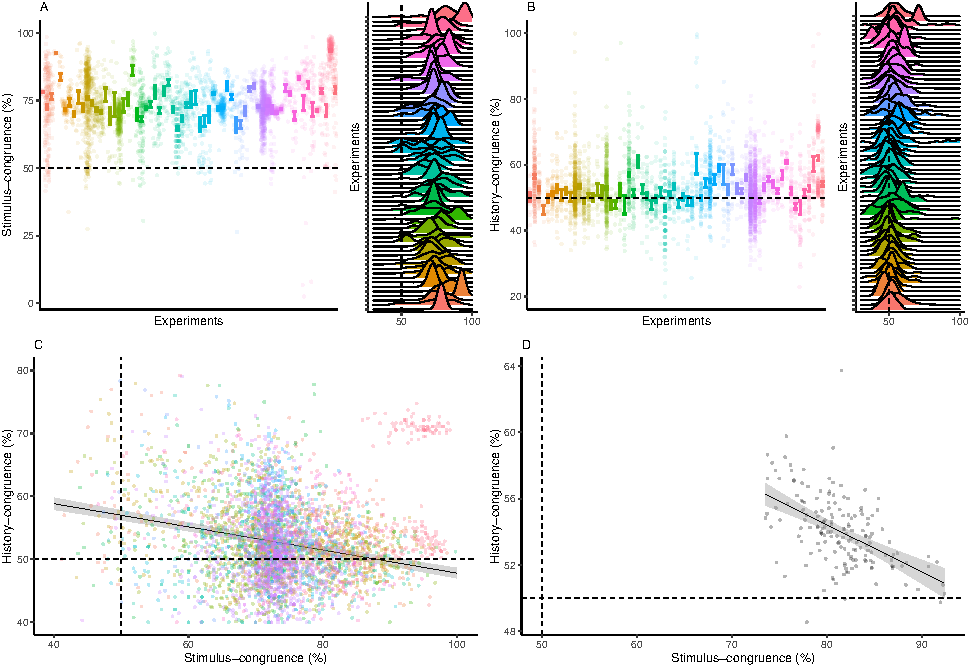
\includegraphics{modes_mouse_rev1b_clean_files/figure-latex/Supplemental_Figure_S1-1.pdf}

\textbf{Supplemental Figure S1. Stimulus- and history-congruence.}

A. Stimulus-congruent choices in humans amounted to 73.46\% ± 0.15\% of
trials and were highly consistent across the experiments selected from
the Confidence Database.

B. History-congruent choices in humans amounted to 52.7\% ± 0.12\% of
trials. In analogy to stimulus-congruence, the prevalence of
history-congruence was highly consistent across the experiments selected
from the Confidence Database. 48.48\% of experiments showed significant
(p \textless{} 0.05) biases toward preceding choices, whereas 2 of the
66 of the included experiments showed significant repelling biases.

C. In humans, we found an enhanced impact of perceptual history in
participants who were less sensitive to external sensory information
(T(\(\ensuremath{4.3\times 10^{3}}\)) = \(-14.27\), p =
\(\ensuremath{3.78\times 10^{-45}}\)), suggesting that perception
results from the competition of external with internal information.

D. In analogy to humans, mice that were less sensitive to external
sensory information showed stronger biases toward perceptual history
(T(163) = -7.52, p = \(\ensuremath{3.44\times 10^{-12}}\), Pearson
correlation).

\newpage

\hypertarget{supplemental-figure-s2}{%
\subsection{Supplemental Figure S2}\label{supplemental-figure-s2}}

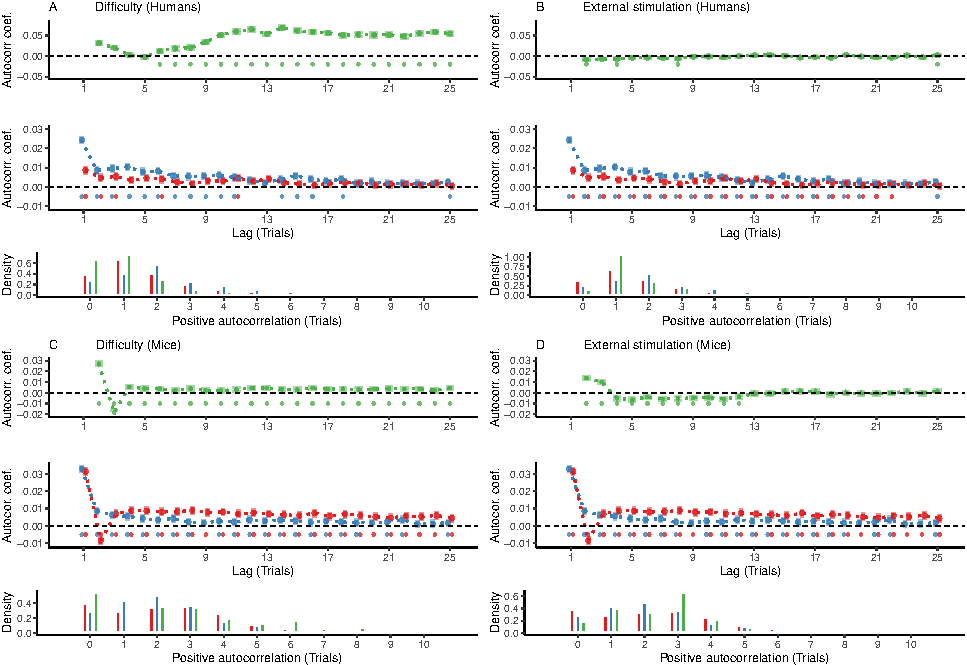
\includegraphics{modes_mouse_rev1b_clean_files/figure-latex/Supplemental_Figure_S2-1.pdf}

\textbf{Supplemental Figure S2. Controlling for task difficulty and
external stimulation.}

In this study, we found highly significant autocorrelations of stimulus-
and history-congruence in humans as well as in mice, while controlling
for task difficulty and the sequence of external stimulation. Here, we
confirm that the autocorrelations of stimulus- and history-congruence
were not a trivial consequence of the experimental design or the
addition of tast difficulty and external stimulation as control
variables in the computation of group-level autocorrelations.

A. In humans, task difficulty (in green) showed a significant
autocorrelation starting at the 5th trial (upper panel, dots at the
bottom indicate intercepts \(\neq\) 0 in trial-wise linear mixed effects
modeling at p \textless{} 0.05). When controlling for task difficulty
only, linear mixed effects modeling indicated a significant
autocorrelation of stimulus-congruence (in red) for the first 3
consecutive trials (middle panel). 20\% of trials within the displayed
time window remained significantly autocorrelated. The autocorrelation
of history-congruence (in blue) remained significant for the first 11
consecutive trials (64\% significantly autocorrelated trials within the
displayed time window). At the level of individual participants, the
autocorrelation of task difficulty exceeded the respective
autocorrelation of randomly permuted within a lag of \(21.66\) ±
\(\ensuremath{8.37\times 10^{-3}}\) trials (lower panel).

B. In humans, the sequence of external stimulation (i.e., which of the
two binary outcomes was supported by the presented stimuli; depicted in
green) was negatively autocorrelated for 1 trial. When controlling for
the autocorrelation of external stimulation only, stimulus-congruence
remained significantly autocorrelated for 22 consecutive trials (88\% of
trials within the displayed time window; lower panel) and
history-congruence remained significantly autocorrelated for 20
consecutive trials (84\% of trials within the displayed time window). At
the level of individual participants, the autocorrelation of external
stimulation exceeded the respective autocorrelation of randomly permuted
within a lag of \(2.94\) ± \(\ensuremath{4.4\times 10^{-3}}\)
consecutive trials (lower panel).

C. In mice, task difficulty showed a significant autocorrelated for the
first 25 consecutive trials (upper panel). When controlling only for
task difficulty only, linear mixed effects modeling indicated a
significant autocorrelation of stimulus-congruence for the first 36
consecutive trials (middle panel). In total, 100\% of trials within the
displayed time window remained significantly autocorrelated. The
autocorrelation of history-congruence remained significant for the first
8 consecutive trials, with 84\% significantly autocorrelated trials
within the displayed time window. At the level of individual mice,
autocorrelation coefficients for difficulty were elevated above randomly
permuted data within a lag of 15.13 ± 0.19 consecutive trials (lower
panel).

D. In mice, the sequence of external stimulation (i.e., which of the two
binary outcomes was supported by the presented stimuli) was negatively
autocorrelated for 11 consecutive trials (upper panel). When controlling
only for the autocorrelation of external stimulation,
stimulus-congruence remained significantly autocorrelated for 86
consecutive trials (100\% of trials within the displayed time window;
middle) and history-congruence remained significantly autocorrelated for
8 consecutive trials (84\% of trials within the displayed time window).
At the level of individual mice, autocorrelation coefficients for
external stimulation were elevated above randomly permuted data within a
lag of \(2.53\) ± \(\ensuremath{9.8\times 10^{-3}}\) consecutive trials
(lower panel).

\newpage

\hypertarget{supplemental-figure-s3}{%
\subsection{Supplemental Figure S3}\label{supplemental-figure-s3}}

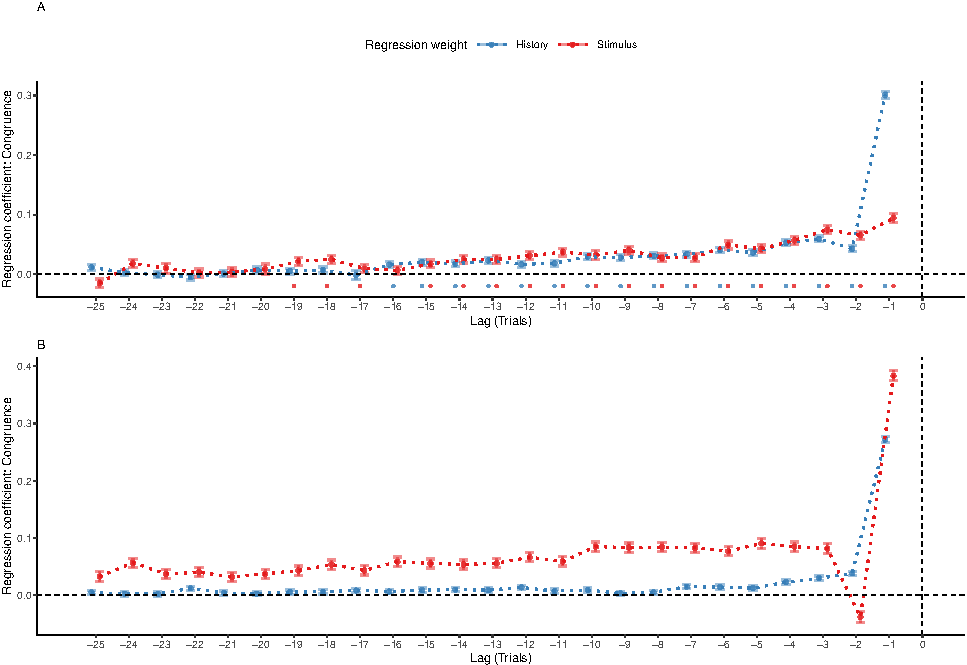
\includegraphics{modes_mouse_rev1b_clean_files/figure-latex/Supplemental_Figure_S3-1.pdf}

\textbf{Supplemental Figure S3. Reproducing group-level autocorrelations
using logistic regression.}

A. As an alternative to group-level autocorrelation coefficients, we
used trial-wise logistic regression to quantify serial dependencies in
stimulus- and history-congruence. This analysis predicted stimulus- and
history-congruence at the index trial (trial \(t = 0\), vertical line)
based on stimulus- and history-congruence at the 100 preceding trials.
Mirroring the shape of the group-level autocorrelations, trial-wise
regression coefficients (depicted as mean ± SEM, dots mark trials with
regression weights significantly greater than zero at p \textless{}
0.05) increased toward the index trial \(t = 0\) for the human data.

B. Following our results in human data, regression coefficients that
predicted history-congruence at the index trial (trial t = 0, vertical
line) increased exponentially for trials closer to the index trial in
mice. In contrast to history-congruence, stimulus-congruence showed a
negative regression weight (or autocorrelation coefficient; Figure 3B)
at trial -2. This was due to the experimental design (see also the
autocorrelations of difficulty and external stimulation in Supplemental
Figure S2C and D): When mice made errors at easy trials (contrast
\(\geq\) 50\%), the upcoming stimulus was shown at the same spatial
location and at high contrast. This increased the probability of
stimulus-congruent perceptual choices after stimulus-incongruent
perceptual choices at easy trials, thereby creating a negative
regression weight (or autocorrelation coefficient) of
stimulus-congruence at trial -2.

\newpage

\hypertarget{supplemental-figure-s4}{%
\subsection{Supplemental Figure S4}\label{supplemental-figure-s4}}

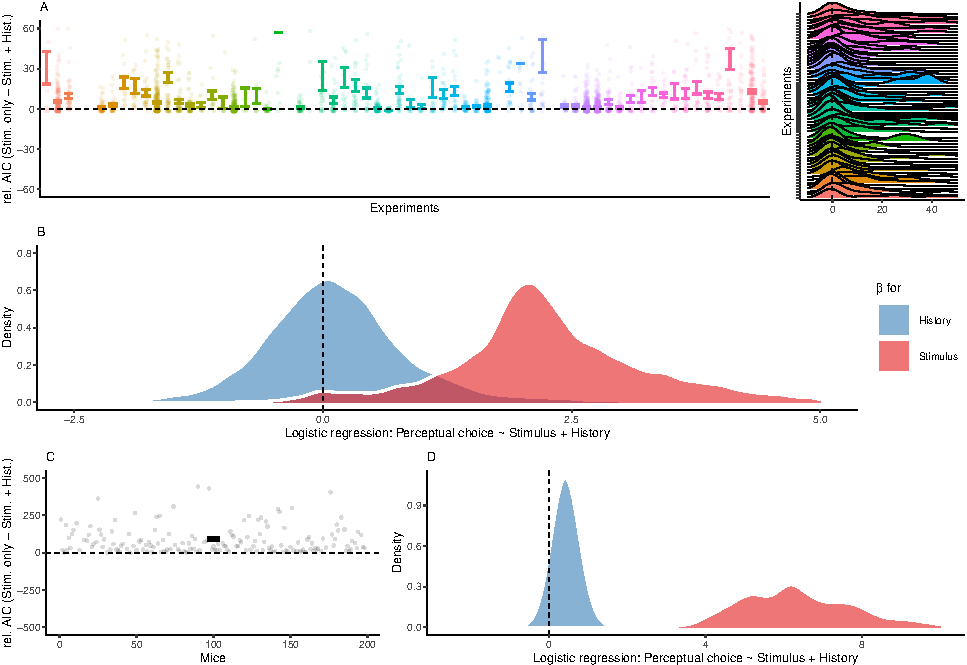
\includegraphics{modes_mouse_rev1b_clean_files/figure-latex/Supplemental_Figure_S4-1.pdf}

\textbf{Supplemental Figure S4. History-congruence in logistic
regression.}

A. To ensure that perceptual history played a significant role in
perception despite the ongoing stream of external information, we tested
whether human perceptual decision-making was better explained by the
combination of external and internal information or, alternatively, by
external information alone. To this end, we compared AIC between
logistic regression models that predicted trial-wise perceptual
responses either by both current external sensory information and the
preceding percept, or by external sensory information alone (values
above zero indicate a superiority of the full model). With high
consistency across the experiments selected from the Confidence
Database, this model-comparison confirmed that perceptual history
contributed significantly to perception (difference in AIC = 8.07 ±
0.53, T(\(57.22\)) = \(4.1\), p = \(\ensuremath{1.31\times 10^{-4}}\)).

B. Participant-wise regression coefficients amount to 0.18 ± 0.02 for
the effect of perceptual history and 2.51 ± 0.03 for external sensory
stimulation.

C. In mice, an AIC-based model comparison indicated that perception was
better explained by logistic regression models that predicted trial-wise
perceptual responses based on both current external sensory information
and the preceding percept (difference in AIC = 88.62 ± 8.57, T(\(164\))
= \(-10.34\), p = \(\ensuremath{1.29\times 10^{-19}}\)).

D. In mice, individual regression coefficients amounted to 0.42 ± 0.02
for the effect of perceptual history and 6.91 ± 0.21 for external
sensory stimulation.

\newpage

\hypertarget{supplemental-figure-s5}{%
\subsection{Supplemental Figure S5}\label{supplemental-figure-s5}}

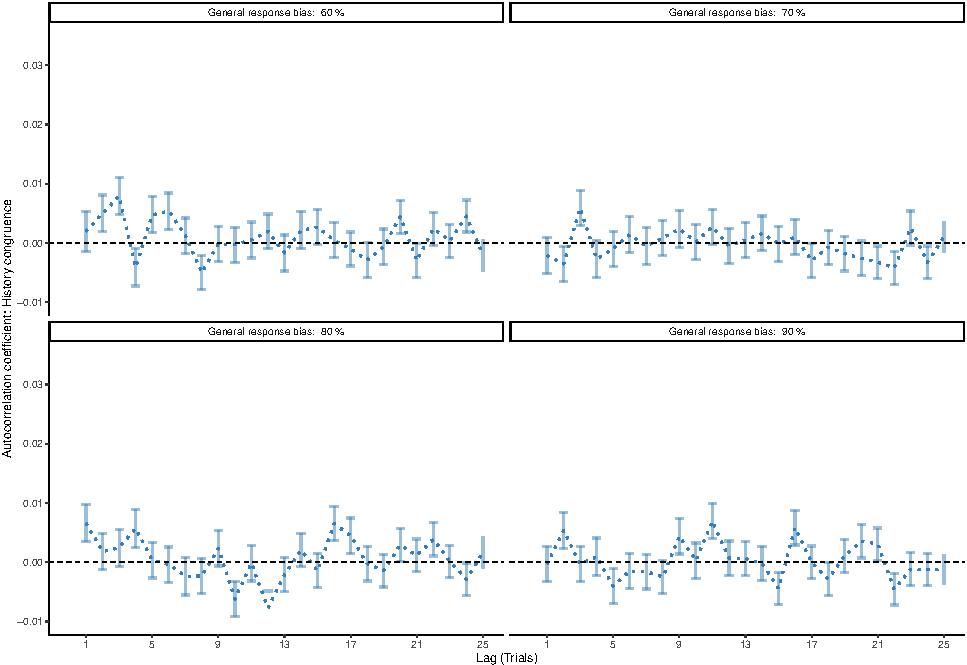
\includegraphics{modes_mouse_rev1b_clean_files/figure-latex/Supplemental_Figure_S5-1.pdf}

\textbf{Supplemental Figure S5. Correcting for general response biases.}

Here, we ask whether the autocorrelation of history-congruence (as shown
in Figure 2-3C) may be driven by general response biases (i.e., a
general propensity to choose one of the two possible outcomes more
frequently than the alternative). To this end, we generated sequences of
100 perceptual choices with general response biases ranging from 60 to
90\% for 1000 simulated participants each. We then computed the
autocorrelation of history-congruence for these simulated data.
Crucially, we used the correction procedure that is applied to the
autocorrelation curves shown in this manuscript: All reported
autocorrelation coefficients are computed relative to the average
autocorrelation coefficients obtained for 100 iterations of randomly
permuted trial sequences. The above simulation show that this correction
procedure removes any potential contribution of general response biases
to the autocorrelation of history-congruence. This indicates that the
autocorrelation of history-congruence (as shown in Figure 2-3C) is not
driven by general response biases that were present in the empirical
data at a level of 58.71\% ± 0.22\% in humans and 54.6\% ± 0.3\% in
mice.

\newpage

\hypertarget{supplemental-figure-s6}{%
\subsection{Supplemental Figure S6}\label{supplemental-figure-s6}}

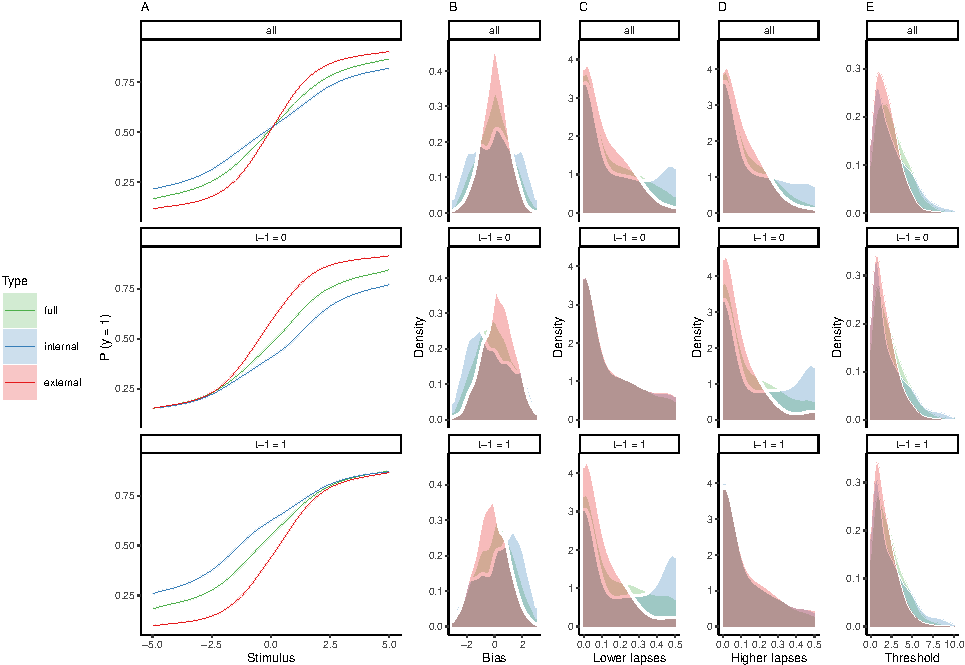
\includegraphics{modes_mouse_rev1b_clean_files/figure-latex/Supplemental_Figure_S6-1.pdf}

\textbf{Supplemental Figure S6. Full and history-conditioned
psychometric functions across modes in humans.}

A. Here, we show average psychometric functions for the full dataset
(upper panel) and conditioned on perceptual history (\(y_{t-1} = 1\) and
\(y_{t-1} = 0\); middle and lower panel) across modes (green line) and
for internal mode (blue line) and external mode (red line) separately.

B. Across the full dataset, biases \(\mu\) were distributed around zero
(\(\beta_0\) = \(\ensuremath{7.37\times 10^{-3}}\) ± \(0.09\),
T(\(36.8\)) = \(0.08\), p = \(0.94\); upper panel), with larger absolute
biases \(|\mu|\) for internal as compared to external mode (\(\beta_0\)
= \(-0.62\) ± \(0.07\), T(\(45.62\)) = \(-8.38\), p =
\(\ensuremath{8.59\times 10^{-11}}\); controlling for differences in
lapses and thresholds). When conditioned on perceptual history, we
observed negative biases for \(y_{t-1} = 0\) (\(\beta_0\) = \(0.56\) ±
\(0.12\), T(\(43.39\)) = \(4.6\), p =
\(\ensuremath{3.64\times 10^{-5}}\); middle panel) and positive biases
for \(y_{t-1} = 1\) (\(\beta_0\) = \(0.56\) ± \(0.12\), T(\(43.39\)) =
\(4.6\), p = \(\ensuremath{3.64\times 10^{-5}}\); lower panel).

C. Lapse rates were higher in internal mode as compared to external mode
(\(\beta_0\) = \(-0.05\) ± \(\ensuremath{5.73\times 10^{-3}}\),
T(\(47.03\)) = \(-9.11\), p = \(\ensuremath{5.94\times 10^{-12}}\);
controlling for differences in biases and thresholds; see upper panel
and subplot D). Importantly, the between-mode difference in lapses
depended on perceptual history: We found no significant difference in
lower lapses \(\gamma\) for \(y_{t-1} = 0\) (\(\beta_0\) = \(0.01\) ±
\(\ensuremath{7.77\times 10^{-3}}\), T(\(33.1\)) = \(1.61\), p =
\(0.12\); middle panel), but a significant difference for
\(y_{t-1} = 1\) (\(\beta_0\) = \(-0.11\) ± \(0.01\), T(\(40.11\)) =
\(-9.59\), p = \(\ensuremath{6.14\times 10^{-12}}\); lower panel).

D. Conversely, higher lapses \(\delta\) were significantly increased for
\(y_{t-1} = 0\) (\(\beta_0\) = \(-0.1\) ±
\(\ensuremath{9.58\times 10^{-3}}\), T(\(36.87\)) = \(-10.16\), p =
\(\ensuremath{3.06\times 10^{-12}}\); middle panel), but not for
\(y_{t-1} = 1\) (\(\beta_0\) = \(0.01\) ±
\(\ensuremath{7.74\times 10^{-3}}\), T(\(33.66\)) = \(1.58\), p =
\(0.12\); lower panel).

E. The thresholds \(t\) were larger in internal as compared to external
mode (\(\beta_0\) = \(-1.77\) ± \(0.25\), T(\(50.45\)) = \(-7.14\), p =
\(\ensuremath{3.48\times 10^{-9}}\); controlling for differences in
biases and lapses) and were not modulated by perceptual history
(\(\beta_0\) = \(0.04\) ± \(0.06\),
T(\(\ensuremath{2.97\times 10^{3}}\)) = \(0.73\), p = \(0.47\)).

\newpage

\hypertarget{supplemental-figure-s7}{%
\subsection{Supplemental Figure S7}\label{supplemental-figure-s7}}

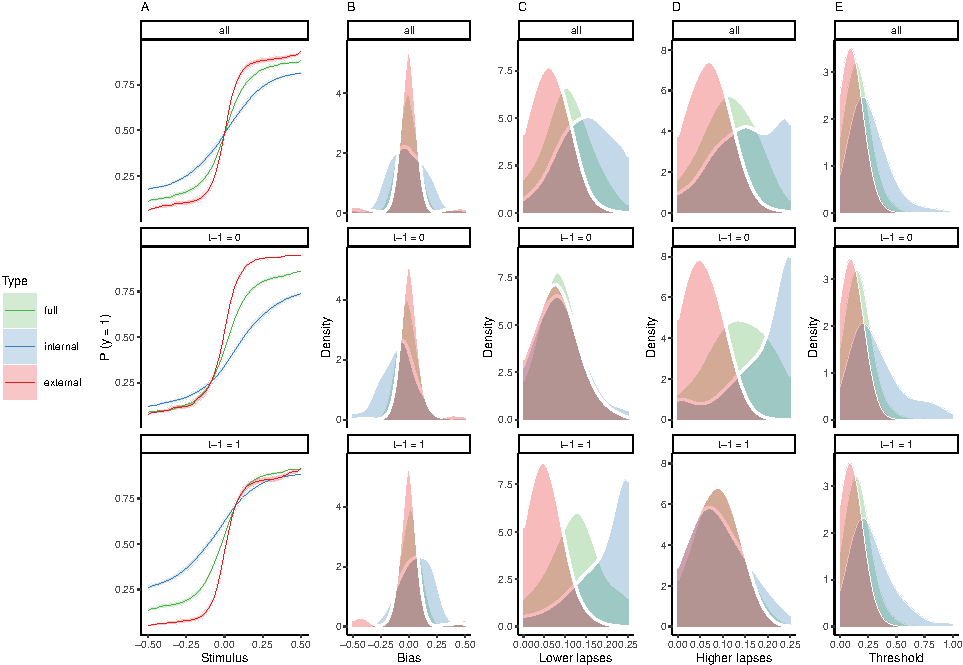
\includegraphics{modes_mouse_rev1b_clean_files/figure-latex/Supplemental_Figure_S7-1.pdf}

\textbf{Supplemental Figure S7. Full and history-conditioned
psychometric functions across modes in mice.}

A. Here, we show average psychometric functions for the full IBL dataset
(upper panel) and conditioned on perceptual history (\(y_{t-1} = 1\) and
\(y_{t-1} = 0\); middle and lower panel) across modes (green line) and
for internal mode (blue line) and external mode (red line) separately.

B. Across the full dataset, biases \(\mu\) were distributed around zero
(T(164) = 0.39, p = \(0.69\); upper panel), with larger absolute biases
\(|\mu|\) for internal as compared to external mode (\(\beta_0\) =
\(-0.18\) ± \(0.03\), T = \(-6.38\), p =
\(\ensuremath{1.77\times 10^{-9}}\); controlling for differences in
lapses and thresholds). When conditioned on perceptual history, we
observed negative biases for \(y_{t-1} = 0\) (T(164) = -1.99, p =
\(0.05\); middle panel) and positive biases for \(y_{t-1} = 1\) (T(164)
= 1.91, p = \(0.06\); lower panel).

C. Lapse rates were higher in internal as compared to external mode
(\(\beta_0\) = \(-0.11\) ± \(\ensuremath{4.39\times 10^{-3}}\), T =
\(-24.8\), p = \(\ensuremath{4.91\times 10^{-57}}\); controlling for
differences in biases and thresholds; upper panel, see subplot D). For
\(y_{t-1} = 1\), the difference between internal and external mode was
more pronounced for lower lapses \(\gamma\) (T(164) = -18.24, p =
\(\ensuremath{2.68\times 10^{-41}}\)) as compared to higher lapses
\(\delta\) (see subplot D). In mice, lower lapses \(\gamma\) were
significantly elevated during internal mode irrespective of the
preceding perceptual choice (middle panel: lower lapses \(\gamma\) for
\(y_{t-1} = 0\); T(164) = -2.5, p = \(0.01\), lower panel: lower lapses
\(\gamma\) for \(y_{t-1} = 1\); T(164) = -32.44, p =
\(\ensuremath{2.92\times 10^{-73}}\)).

D. For \(y_{t-1} = 0\), the difference between internal and external
mode was more pronounced for higher lapses \(\delta\) (T(164) = 21.44, p
= \(\ensuremath{1.93\times 10^{-49}}\), see subplot C). Higher lapses
were significantly elevated during internal mode irrespective of the
preceding perceptual choice (middle panel: higher lapses \(\delta\) for
\(y_{t-1} = 0\); T(164) = -28.29, p =
\(\ensuremath{5.62\times 10^{-65}}\) lower panel: higher lapses
\(\delta\) for \(y_{t-1} = 1\); T(164) = -2.65, p =
\(\ensuremath{8.91\times 10^{-3}}\); ).

E. Thresholds \(t\) were higher in internal as compared to external mode
(\(\beta_0\) = \(-0.28\) ± \(0.04\), T = \(-7.26\), p =
\(\ensuremath{1.53\times 10^{-11}}\); controlling for differences in
biases and lapses) and were not modulated by perceptual history (T(164)
= 0.94, p = \(0.35\)).

\newpage

\hypertarget{supplemental-figure-s8}{%
\subsection{Supplemental Figure S8}\label{supplemental-figure-s8}}

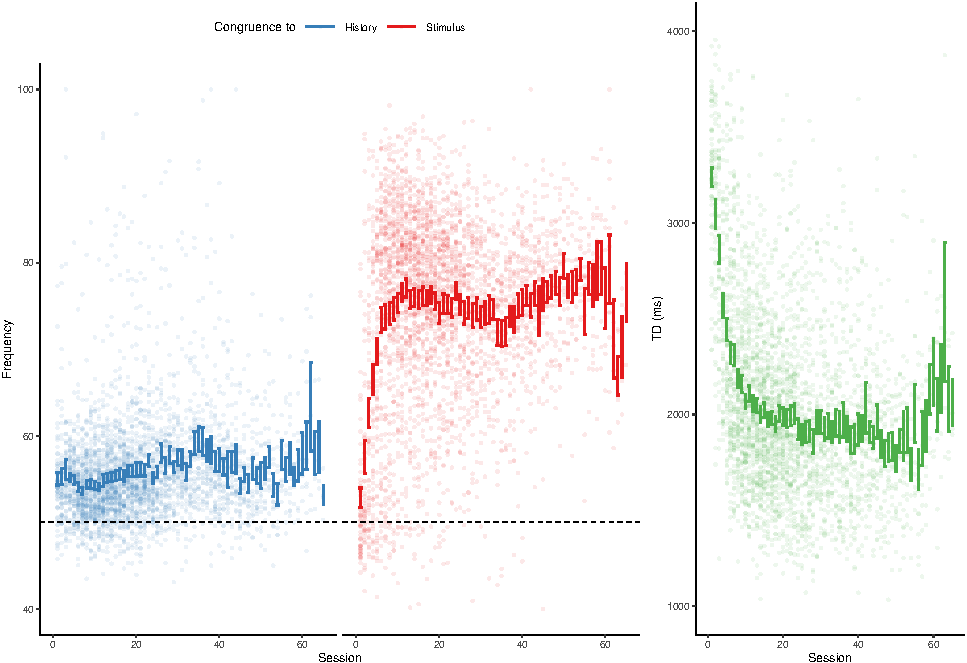
\includegraphics{modes_mouse_rev1b_clean_files/figure-latex/Supplemental_Figure_S8-1.pdf}

\textbf{Supplemental Figure S8. History-/stimulus-congruence and TDs
during training of the basic task.}

Here, we depict the progression of history- and stimulus-congruence
(depicted in blue and red, respectively; left panel) as well as TDs (in
green; right panel) across training sessions in mice that achieved
proficiency (i.e., stimulus-congruence \(\geq\) 80\%) in the
\emph{basic} task of the IBL dataset. We found that both
history-congruent perceptual choices (\(\beta\) = \(0.13\) ±
\(\ensuremath{4.67\times 10^{-3}}\),
T(\(\ensuremath{8.4\times 10^{3}}\)) = \(27.04\), p =
\(\ensuremath{1.96\times 10^{-154}}\)) and stimulus-congruent perceptual
choices (\(\beta\) = \(0.34\) ± \(\ensuremath{7.13\times 10^{-3}}\),
T(\(\ensuremath{8.51\times 10^{3}}\)) = \(47.66\), p < \(\ensuremath{2.2\times 10^{-308}}\)) became
more frequent with training. As in humans, mice showed shorter TDs with
increased exposure to the task (\(\beta\) = \(-22.14\) ± \(17.06\),
T(\(\ensuremath{1.14\times 10^{3}}\)) = \(-1.3\), p < \(\ensuremath{2.2\times 10^{-308}}\)).

\newpage

\hypertarget{supplemental-figure-s9}{%
\subsection{Supplemental Figure S9}\label{supplemental-figure-s9}}

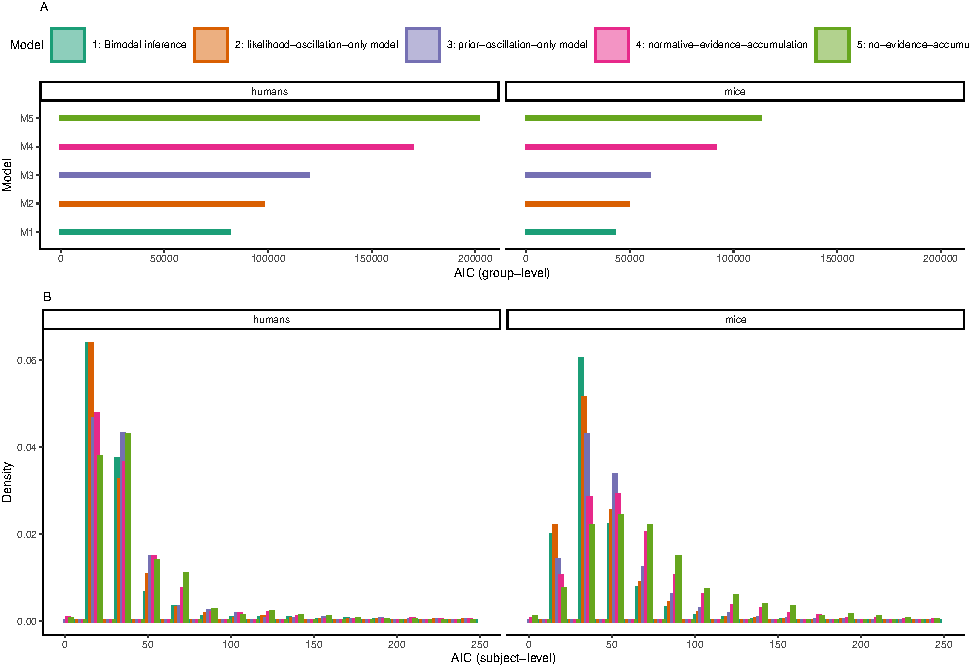
\includegraphics{modes_mouse_rev1b_clean_files/figure-latex/Supplemental_Figure_S9-1.pdf}
\textbf{Supplemental Figure S9. Comparison of the bimodal inference
model against reduced control models.}

A. Group-level AIC. The bimodal inference model (M1) achieved the lowest
AIC across the full model space (\(AIC_1\) =
\(\ensuremath{8.16\times 10^{4}}\) in humans and
\(\ensuremath{4.24\times 10^{4}}\) in mice). Model M2 (\(AIC_2\) =
\(\ensuremath{9.76\times 10^{4}}\) in humans and
\(\ensuremath{4.91\times 10^{4}}\) in mice) and Model M3 (\(AIC_3\) =
\(\ensuremath{1.19\times 10^{5}}\) in humans and
\(\ensuremath{5.95\times 10^{4}}\) in mice) incorporated only
oscillations of either likelihood or prior precision. Model M4
(\(AIC_4\) = \(\ensuremath{1.69\times 10^{5}}\) in humans and
\(\ensuremath{9.12\times 10^{4}}\) in mice) lacked any oscillations of
likelihood and prior precision and corresponded to the normative model
proposed by Glaze et al.\textsuperscript{51}. In model M5 (\(AIC_4\) =
\(\ensuremath{2.01\times 10^{5}}\) in humans and
\(\ensuremath{1.13\times 10^{5}}\) in mice), we furthermore removed the
integration of information across trials, such that perception depended
only in incoming sensory information.

B. Subject-level AIC. Here, we show the distribution of AIC values at
the subject-level. AIC for the bimodal inference model tended to be
smaller than AIC for the comparator models (statistical comparison to
the second-best model M2 in humans: \(\beta\) = \(-1.71\) ± \(0.19\),
T(\(\ensuremath{8.57\times 10^{3}}\)) = \(-8.85\), p =
\(\ensuremath{1.06\times 10^{-18}}\); mice:
T(\(\ensuremath{1.57\times 10^{3}}\)) = -3.08, p =
\(\ensuremath{2.12\times 10^{-3}}\)).

\newpage

\hypertarget{supplemental-figure-s10}{%
\subsection{Supplemental Figure S10}\label{supplemental-figure-s10}}

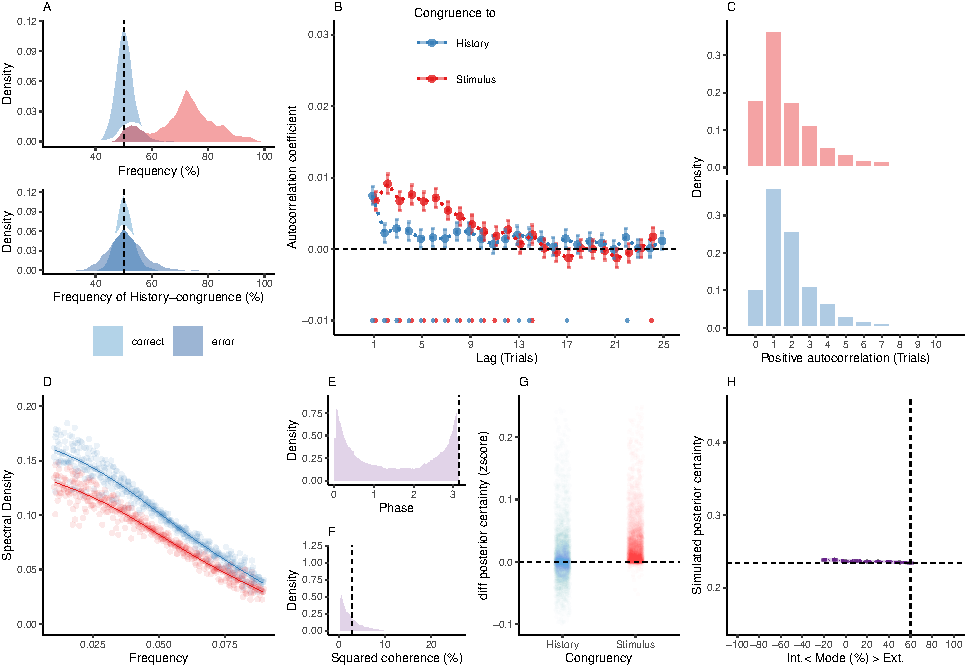
\includegraphics{modes_mouse_rev1b_clean_files/figure-latex/Supplemental_Figure_S10-1.pdf}

\textbf{Supplemental Figure S10. Reduced Control Model M2: Only
oscillation of the likelihood.} When simulating data for the
\emph{likelihood-oscillation-only model}, we removed the oscillation
from the prior term by setting the amplitude \(a_{\psi}\) to zero.
Simulated data thus depended only on the participant-wise estimates for
hazard rate \(H\), amplitude \(a_{LLR}\), frequency \(f\), phase \(p\)
and inverse decision temperature \(\zeta\).

A. Similar to the full model M1 (Figure 1F and Figure 4), simulated
perceptual choices were stimulus-congruent in 71.97\% ± 0.17\% of trials
(in red). History-congruent amounted to 50.76\% ± 0.07\% of trials (in
blue). As in the full model, the likelihood-oscillation-only model
showed a significant bias toward perceptual history
T(\ensuremath{4.32\times 10^{3}}) = 10.29, p =
\(\ensuremath{1.54\times 10^{-24}}\); upper panel). Similarly,
history-congruent choices were more frequent at error trials
(T(\ensuremath{4.32\times 10^{3}}) = 9.71, p =
\(\ensuremath{4.6\times 10^{-22}}\); lower panel).

B. In the likelihood-oscillation-only model, we observed that the
autocorrelation coefficients for history-congruence were reduced below
the autocorrelation coefficients of stimulus-congruence. This is an
approximately five-fold reduction relative to the empirical results
observed in humans (Figure 2B), where the autocorrelation of
history-congruence was above the autocorrelation of stimulus-congruence.
Moreover, in the reduced model shown here, the number of consecutive
trials that showed significant autocorrelation of history-congruence was
reduced to 11.

C. In the likelihood-oscillation-only model, the number of consecutive
trials at which true autocorrelation coefficients exceeded the
autocorrelation coefficients for randomly permuted data did not differ
with respect to stimulus-congruence (2.62 ±
\ensuremath{1.39\times 10^{-3}} trials;
T(\ensuremath{4.32\times 10^{3}}) = 1.85, p = \(0.06\)), but decreased
with respect to history-congruence (2.4 ±
\ensuremath{8.45\times 10^{-4}} trials;
T(\ensuremath{4.32\times 10^{3}}) = -15.26, p =
\(\ensuremath{3.11\times 10^{-51}}\)) relative to the full model.

D. In the likelihood-oscillation-only model, the smoothed probabilities
of stimulus- and history-congruence (sliding windows of ±5 trials)
fluctuated as a scale-invariant process with a 1/f power law, i.e., at
power densities that were inversely proportional to the frequency (power
\textasciitilde{} 1/\(f^\beta\); stimulus-congruence: \(\beta\) =
\(-0.81\) ± \(\ensuremath{1.17\times 10^{-3}}\),
T(\(\ensuremath{1.92\times 10^{5}}\)) = \(-688.65\), p < \(\ensuremath{2.2\times 10^{-308}}\);
history-congruence: \(\beta\) = \(-0.79\) ±
\(\ensuremath{1.14\times 10^{-3}}\),
T(\(\ensuremath{1.92\times 10^{5}}\)) = \(-698.13\), p < \(\ensuremath{2.2\times 10^{-308}}\)).

E. In the likelihood-oscillation-only model, the distribution of phase
shift between fluctuations in simulated stimulus- and history-congruence
peaked at half a cycle (\(\pi\) denoted by dotted line). In contrast to
the full model, the dynamic probabilities of simulated stimulus- and
history-congruence were positively correlated (\(\beta\) =
\(\ensuremath{2.7\times 10^{-3}}\) ± \(\ensuremath{7.6\times 10^{-4}}\),
T(\(\ensuremath{2.02\times 10^{6}}\)) = \(3.55\), p =
\(\ensuremath{3.8\times 10^{-4}}\)).

F. In the likelihood-oscillation-only model, the average squared
coherence between fluctuations in simulated stimulus- and
history-congruence (black dotted line) was reduced in comparison to the
full model (T(\ensuremath{3.51\times 10^{3}}) = -4.56, p =
\(\ensuremath{5.27\times 10^{-6}}\)) and amounted to 3.43 ±
\ensuremath{1.02\times 10^{-3}}\%.

G. Similar to the full bimodal inference model, confidence simulated
from the likelihood-oscillation-only model was enhanced for
stimulus-congruent choices (\(\beta\) = \(0.03\) ±
\(\ensuremath{1.42\times 10^{-4}}\),
T(\(\ensuremath{2.1\times 10^{6}}\)) = \(191.78\), p < \(\ensuremath{2.2\times 10^{-308}}\)) and
history-congruent choices (\(\beta\) =
\(\ensuremath{9.1\times 10^{-3}}\) ±
\(\ensuremath{1.25\times 10^{-4}}\),
T(\(\ensuremath{2.1\times 10^{6}}\)) = \(72.51\), p < \(\ensuremath{2.2\times 10^{-308}}\)).

H. In the likelihood-oscillation-only model, the positive quadratic
relationship between the mode of perceptual processing and confidence
was markedly reduced in comparison to the full model (\(\beta_2\) =
\(0.34\) ± \(0.1\), T(\(\ensuremath{2.1\times 10^{6}}\)) = \(3.49\), p =
\(\ensuremath{4.78\times 10^{-4}}\)). The horizontal and vertical dotted
lines indicate minimum posterior certainty and the associated mode,
respectively.

\newpage

\hypertarget{supplemental-figure-s11}{%
\subsection{Supplemental Figure S11}\label{supplemental-figure-s11}}

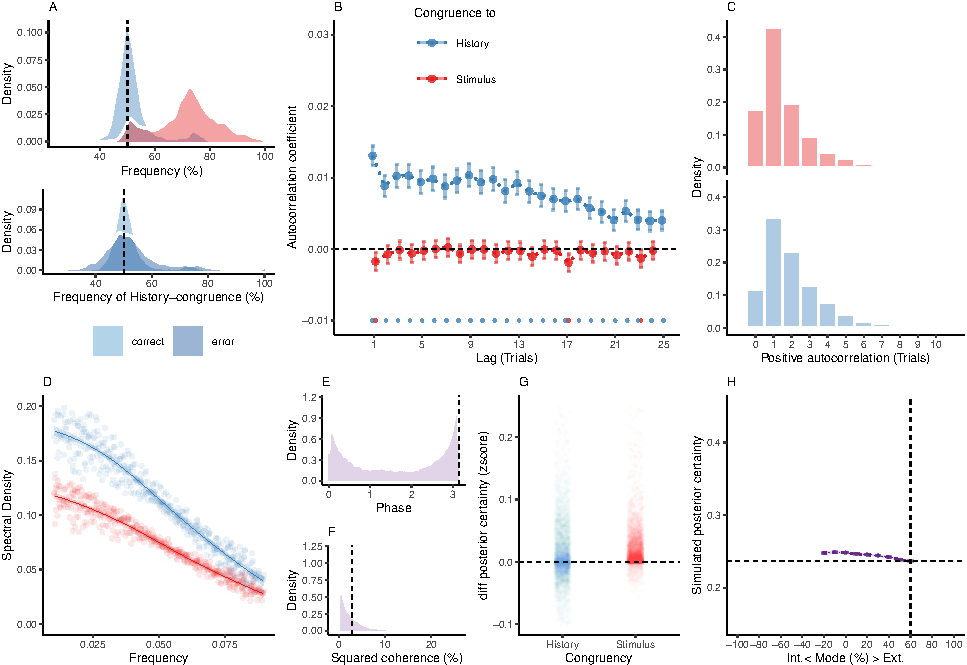
\includegraphics{modes_mouse_rev1b_clean_files/figure-latex/Supplemental_Figure_S11-1.pdf}

\textbf{Supplemental Figure S11. Reduced Control Model M3: Only
oscillation of the prior.} When simulating data for the
\emph{prior-oscillation-only model}, we removed the oscillation from the
prior term by setting the amplitude \(a_{LLR}\) to zero. Simulated data
thus depended only on the participant-wise estimates for hazard rate
\(H\), amplitude \(a_{\psi}\), frequency \(f\), phase \(p\) and inverse
decision temperature \(\zeta\).

A. Similar to the full model (Figure 1F and Figure 4), simulated
perceptual choices were stimulus-congruent in 71.97\% ± 0.17\% of trials
(in red). History-congruent amounted to 52.1\% ± 0.11\% of trials (in
blue). As in the full model, the prior-oscillation-only showed a
significant bias toward perceptual history
T(\ensuremath{4.32\times 10^{3}}) = 18.34, p =
\(\ensuremath{1.98\times 10^{-72}}\); upper panel). Similarly,
history-congruent choices were more frequent at error trials
(T(\ensuremath{4.31\times 10^{3}}) = 12.35, p =
\(\ensuremath{1.88\times 10^{-34}}\); lower panel).

B. In the prior-oscillation-only model, we did not observe any
significant positive autocorrelation of stimulus-congruence , whereas
the autocorrelation of history-congruence was preserved.

C. In the prior-oscillation-only model, the number of consecutive trials
at which true autocorrelation coefficients exceeded the autocorrelation
coefficients for randomly permuted data did was decreased with respect
to stimulus-congruence relative to the full model (1.8 ±
\ensuremath{1.01\times 10^{-3}} trials;
T(\ensuremath{4.31\times 10^{3}}) = -6.48, p =
\(\ensuremath{1.03\times 10^{-10}}\)), but did not differ from the full
model with respect to history-congruence (4.25 ±
\ensuremath{1.84\times 10^{-3}} trials;
T(\ensuremath{4.32\times 10^{3}}) = 0.07, p = \(0.95\)).

D. In the prior-oscillation-only model, the smoothed probabilities of
stimulus- and history-congruence (sliding windows of ±5 trials)
fluctuated as a scale-invariant process with a 1/f power law, i.e., at
power densities that were inversely proportional to the frequency (power
\textasciitilde{} 1/\(f^\beta\); stimulus-congruence: \(\beta\) =
\(-0.78\) ± \(\ensuremath{1.11\times 10^{-3}}\),
T(\(\ensuremath{1.92\times 10^{5}}\)) = \(-706.62\), p < \(\ensuremath{2.2\times 10^{-308}}\);
history-congruence: \(\beta\) = \(-0.83\) ±
\(\ensuremath{1.27\times 10^{-3}}\),
T(\(\ensuremath{1.92\times 10^{5}}\)) = \(-651.6\), p < \(\ensuremath{2.2\times 10^{-308}}\)).

E. In the prior-oscillation-only model, the distribution of phase shift
between fluctuations in simulated stimulus- and history-congruence
peaked at half a cycle (\(\pi\) denoted by dotted line). Similar to the
full model, the dynamic probabilities of simulated stimulus- and
history-congruence were anti-correlated (\(\beta\) = \(-0.03\) ±
\(\ensuremath{8.61\times 10^{-4}}\),
T(\(\ensuremath{2.12\times 10^{6}}\)) = \(-34.03\), p =
\(\ensuremath{8.17\times 10^{-254}}\)).

F. In the prior-oscillation-only model, the average squared coherence
between fluctuations in simulated stimulus- and history-congruence
(black dotted line) was reduced in comparison to the full model
(T(\ensuremath{3.54\times 10^{3}}) = -3.22, p =
\(\ensuremath{1.28\times 10^{-3}}\)) and amounted to 3.52 ±
\ensuremath{1.04\times 10^{-3}}\%.

G. Similar to the full bimodal inference model, confidence simulated
from the prior-oscillation-only model was enhanced for
stimulus-congruent choices (\(\beta\) = \(0.02\) ±
\(\ensuremath{1.44\times 10^{-4}}\),
T(\(\ensuremath{2.03\times 10^{6}}\)) = \(128.53\), p < \(\ensuremath{2.2\times 10^{-308}}\)) and
history-congruent choices (\(\beta\) = \(0.01\) ±
\(\ensuremath{1.26\times 10^{-4}}\),
T(\(\ensuremath{2.03\times 10^{6}}\)) = \(88.24\), p < \(\ensuremath{2.2\times 10^{-308}}\)).

H. In contrast to the full bimodal inference model, the
prior-oscillation-only model did not yield a positive quadratic
relationship between the mode of perceptual processing and confidence
(\(\beta_2\) = \(-0.17\) ± \(0.1\),
T(\(\ensuremath{2.04\times 10^{6}}\)) = \(-1.66\), p = \(0.1\)). The
horizontal and vertical dotted lines indicate minimum posterior
certainty and the associated mode, respectively.

\newpage

\hypertarget{supplemental-figure-s12}{%
\subsection{Supplemental Figure S12}\label{supplemental-figure-s12}}

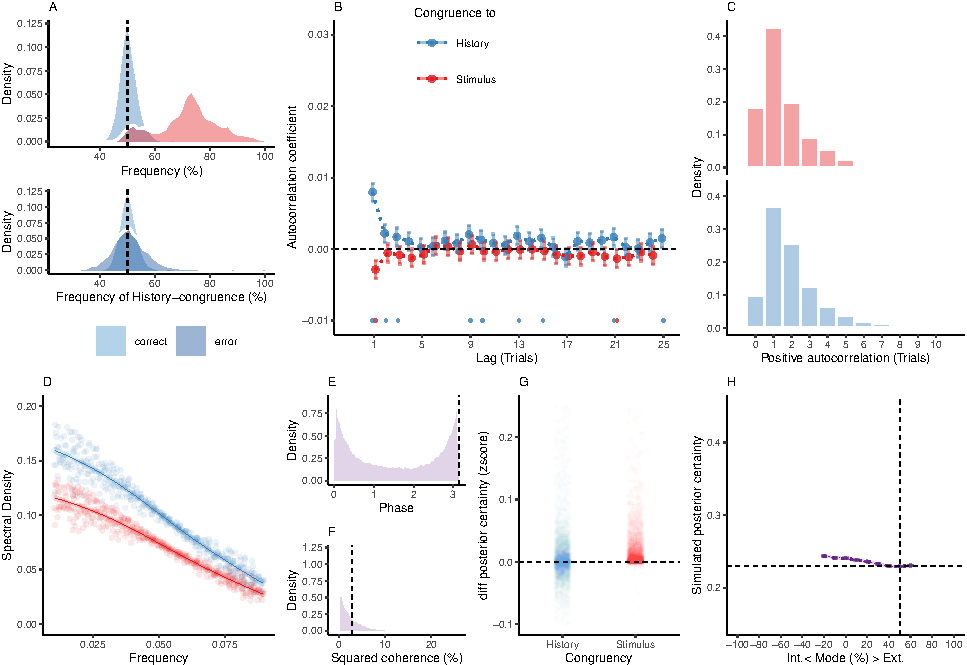
\includegraphics{modes_mouse_rev1b_clean_files/figure-latex/Supplemental_Figure_S12-1.pdf}

\textbf{Supplemental Figure S12. Reduced Control Model M4: Normative
evidence accumulation.} When simulating data for the
\emph{normative-evidence-accumulation model}, we removed the oscillation
from the likelihood and prior terms by setting the amplitudes
\(a_{LLR}\) and \(a_{\psi}\) to zero. Simulated data thus depended only
on the participant-wise estimates for hazard rate \(H\) and inverse
decision temperature \(\zeta\).

A. Similar to the full model (Figure 1F and Figure 4), simulated
perceptual choices were stimulus-congruent in 71.97\% ± 0.17\% of trials
(in red). History-congruent amounted to 50.73\% ± 0.07\% of trials (in
blue). As in the full model, the no-oscillation model showed a
significant bias toward perceptual history
T(\ensuremath{4.32\times 10^{3}}) = 9.94, p =
\(\ensuremath{4.88\times 10^{-23}}\); upper panel). Similarly,
history-congruent choices were more frequent at error trials
(T(\ensuremath{4.31\times 10^{3}}) = 10.59, p =
\(\ensuremath{7.02\times 10^{-26}}\); lower panel).

B. In the normative-evidence-accumulation model, we did not find
significant autocorrelations for stimulus-congruence. Likewise, we did
not observe any autocorrelation of history-congruence beyond the first
three consecutive trials.

C. In the normative-evidence-accumulation model, the number of
consecutive trials at which true autocorrelation coefficients exceeded
the autocorrelation coefficients for randomly permuted data decreased
with respect to both stimulus-congruence (1.8 ±
\ensuremath{1.59\times 10^{-3}} trials;
T(\ensuremath{4.31\times 10^{3}}) = -5.21, p =
\(\ensuremath{2\times 10^{-7}}\)) and history-congruence (2.18 ±
\ensuremath{5.48\times 10^{-4}} trials;
T(\ensuremath{4.32\times 10^{3}}) = -17.1, p =
\(\ensuremath{1.75\times 10^{-63}}\)) relative to the full model.

D. In the normative-evidence-accumulation model, the smoothed
probabilities of stimulus- and history-congruence (sliding windows of ±5
trials) fluctuated as a scale-invariant process with a 1/f power law,
i.e., at power densities that were inversely proportional to the
frequency (power \textasciitilde{} 1/\(f^\beta\); stimulus-congruence:
\(\beta\) = \(-0.78\) ± \(\ensuremath{1.1\times 10^{-3}}\),
T(\(\ensuremath{1.92\times 10^{5}}\)) = \(-706.93\), p < \(\ensuremath{2.2\times 10^{-308}}\);
history-congruence: \(\beta\) = \(-0.79\) ±
\(\ensuremath{1.12\times 10^{-3}}\),
T(\(\ensuremath{1.92\times 10^{5}}\)) = \(-702.46\), p < \(\ensuremath{2.2\times 10^{-308}}\)).

E. In the normative-evidence-accumulation model, the distribution of
phase shift between fluctuations in simulated stimulus- and
history-congruence peaked at half a cycle (\(\pi\) denoted by dotted
line). In contrast to the full model, the dynamic probabilities of
simulated stimulus- and history-congruence were positively correlated
(\(\beta\) = \(\ensuremath{4.3\times 10^{-3}}\) ±
\(\ensuremath{7.97\times 10^{-4}}\),
T(\(\ensuremath{1.98\times 10^{6}}\)) = \(5.4\), p =
\(\ensuremath{6.59\times 10^{-8}}\)).

F. In the normative-evidence-accumulation model, the average squared
coherence between fluctuations in simulated stimulus- and
history-congruence (black dotted line) was reduced in comparison to the
full model (T(\ensuremath{3.52\times 10^{3}}) = -6.27, p =
\(\ensuremath{3.97\times 10^{-10}}\)) and amounted to 3.26 ±
\ensuremath{8.88\times 10^{-4}}\%.

G. Similar to the full bimodal inference model, confidence simulated
from the no-oscillation model was enhanced for stimulus-congruent
choices (\(\beta\) = \(0.01\) ± \(\ensuremath{1.05\times 10^{-4}}\),
T(\(\ensuremath{2.1\times 10^{6}}\)) = \(139.17\), p < \(\ensuremath{2.2\times 10^{-308}}\)) and
history-congruent choices (\(\beta\) =
\(\ensuremath{8.05\times 10^{-3}}\) ±
\(\ensuremath{9.2\times 10^{-5}}\), T(\(\ensuremath{2.1\times 10^{6}}\))
= \(87.54\), p < \(\ensuremath{2.2\times 10^{-308}}\)).

H. In the normative-evidence-accumulation model, the positive quadratic
relationship between the mode of perceptual processing and confidence
was markedly reduced in comparison to the full model (\(\beta_2\) =
\(0.14\) ± \(0.07\), T(\(\ensuremath{2.1\times 10^{6}}\)) = \(1.95\), p
= \(0.05\)). The horizontal and vertical dotted lines indicate minimum
posterior certainty and the associated mode, respectively.

\newpage

\hypertarget{supplemental-figure-s13}{%
\subsection{Supplemental Figure S13}\label{supplemental-figure-s13}}

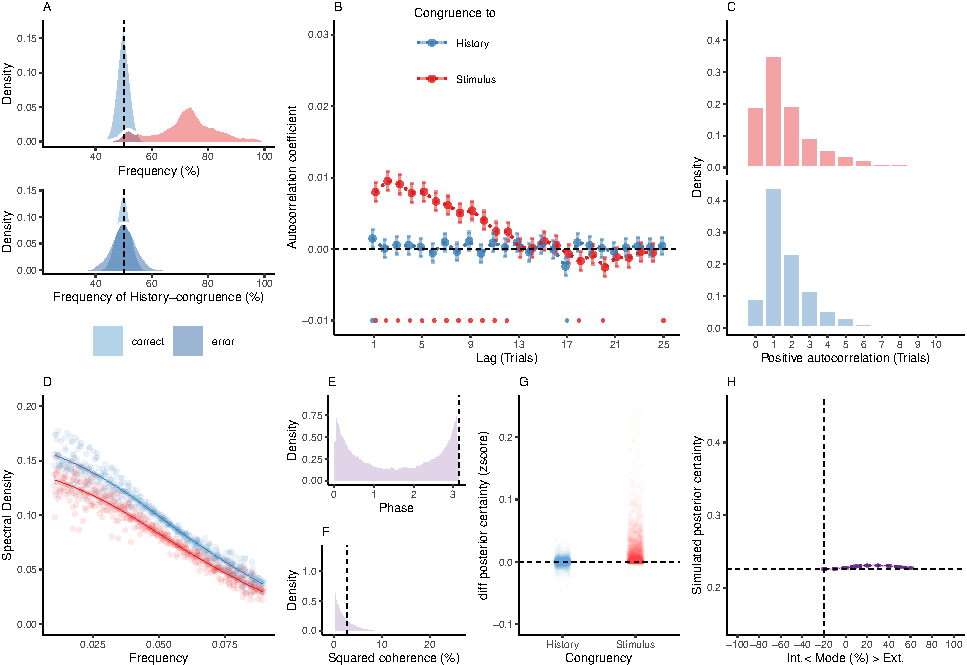
\includegraphics{modes_mouse_rev1b_clean_files/figure-latex/Supplemental_Figure_13-1.pdf}

\textbf{Supplemental Figure S13. Reduced Control Model M5: No
accumulation of information across trials.} When simulating data for the
\emph{no-evidence-accumulation model}, we removed the accumulation of
information across trials by setting the Hazard rate \(H\) to 0.5.
Simulated data thus depended only on the participant-wise estimates for
the amplitudes \(a_{LLR/\psi}\), frequency \(f\), phase \(p\) and
inverse decision temperature \(\zeta\).

A. Similar to the full model (Figure 1F and Figure 4), simulated
perceptual choices were stimulus-congruent in 72.14\% ± 0.17\% of trials
(in red). History-congruent amounted to 49.89\% ± 0.03\% of trials (in
blue). In contrast to the full model, the no-accumulation model showed a
significant bias against perceptual history
T(\ensuremath{4.32\times 10^{3}}) = -3.28, p =
\(\ensuremath{1.06\times 10^{-3}}\); upper panel). In contrast to the
full model, there was no difference in the frequency of
history-congruent choices between correct and error trials
(T(\ensuremath{4.31\times 10^{3}}) = 0.76, p = \(0.44\); lower panel).

B. In the no-evidence-accumulation model, we found no significant
autocorrelation of history-congruence beyond the first trial, whereas
the autocorrelation of stimulus-congruence was preserved.

C. In the no-evidence-accumulation model, the number of consecutive
trials at which true autocorrelation coefficients exceeded the
autocorrelation coefficients for randomly permuted data increased with
respect to stimulus-congruence (2.83 ± \ensuremath{1.49\times 10^{-3}}
trials; T(\ensuremath{4.31\times 10^{3}}) = 3.45, p =
\(\ensuremath{5.73\times 10^{-4}}\)) and decreased with respect to
history-congruence (1.85 ± \ensuremath{3.49\times 10^{-4}} trials;
T(\ensuremath{4.32\times 10^{3}}) = -19.37, p =
\(\ensuremath{3.49\times 10^{-80}}\)) relative to the full model.

D. In the no-evidence-accumulation model, the smoothed probabilities of
stimulus- and history-congruence (sliding windows of ±5 trials)
fluctuated as a scale-invariant process with a 1/f power law, i.e., at
power densities that were inversely proportional to the frequency (power
\textasciitilde{} 1/\(f^\beta\); stimulus-congruence: \(\beta\) =
\(-0.82\) ± \(\ensuremath{1.2\times 10^{-3}}\),
T(\(\ensuremath{1.92\times 10^{5}}\)) = \(-681.98\), p < \(\ensuremath{2.2\times 10^{-308}}\);
history-congruence: \(\beta\) = \(-0.78\) ±
\(\ensuremath{1.11\times 10^{-3}}\),
T(\(\ensuremath{1.92\times 10^{5}}\)) = \(-706.57\), p < \(\ensuremath{2.2\times 10^{-308}}\)).

E. In the no-evidence-accumulation model, the distribution of phase
shift between fluctuations in simulated stimulus- and history-congruence
peaked at half a cycle (\(\pi\) denoted by dotted line). In contrast to
the full model, the dynamic probabilities of simulated stimulus- and
history-congruence were not significantly anti-correlated (\(\beta\) =
\(\ensuremath{6.39\times 10^{-4}}\) ±
\(\ensuremath{7.22\times 10^{-4}}\),
T(\(\ensuremath{8.89\times 10^{5}}\)) = \(0.89\), p = \(0.38\)).

F. In the no-evidence-accumulation model, the average squared coherence
between fluctuations in simulated stimulus- and history-congruence
(black dotted line) was reduced in comparison to the full model
(T(\ensuremath{3.56\times 10^{3}}) = -9.96, p =
\(\ensuremath{4.63\times 10^{-23}}\)) and amounted to 2.8 ±
\ensuremath{7.29\times 10^{-4}}\%.

G. Similar to the full bimodal inference model, confidence simulated
from the no-evidence-accumulation model was enhanced for
stimulus-congruent choices (\(\beta\) = \(0.01\) ±
\(\ensuremath{9.4\times 10^{-5}}\),
T(\(\ensuremath{2.11\times 10^{6}}\)) = \(158.1\), p < \(\ensuremath{2.2\times 10^{-308}}\)). In
contrast to the full bimodal inference model, history-congruent choices
were not characterized by enhanced confidence (\(\beta\) =
\(\ensuremath{8.78\times 10^{-5}}\) ±
\(\ensuremath{8.21\times 10^{-5}}\),
T(\(\ensuremath{2.11\times 10^{6}}\)) = \(1.07\), p = \(0.29\)).

H. In the no-evidence-accumulation model, the positive quadratic
relationship between the mode of perceptual processing and confidence
was markedly reduced in comparison to the full model (\(\beta_2\) =
\(0.19\) ± \(0.06\), T(\(\ensuremath{2.11\times 10^{6}}\)) = \(3\), p =
\(\ensuremath{2.69\times 10^{-3}}\)). The horizontal and vertical dotted
lines indicate minimum posterior certainty and the associated mode,
respectively.

\newpage

\hypertarget{supplemental-figure-s14}{%
\subsection{Supplemental Figure S14}\label{supplemental-figure-s14}}

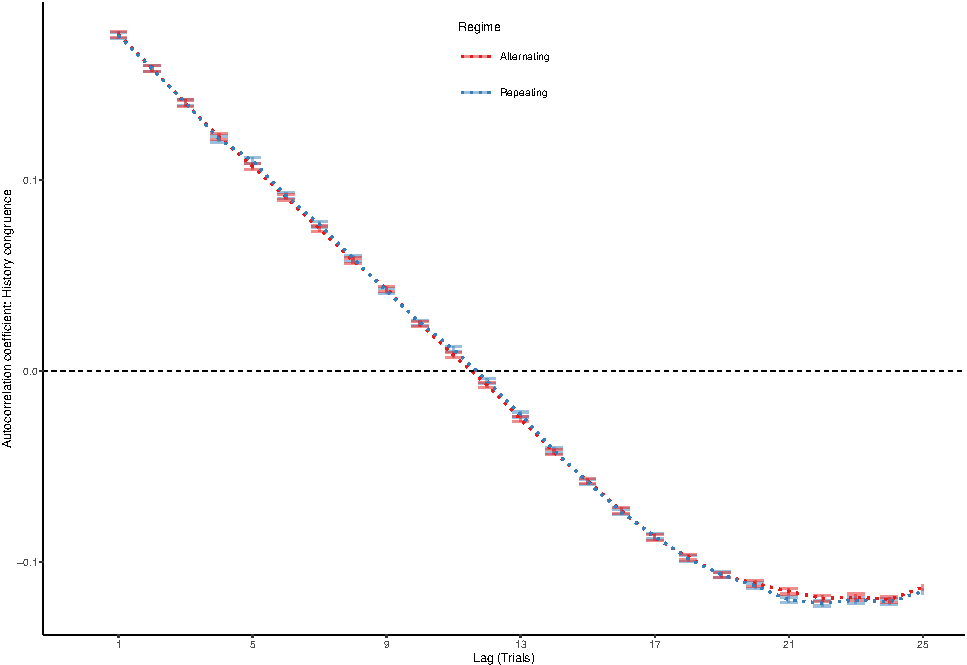
\includegraphics{modes_mouse_rev1b_clean_files/figure-latex/Supplemental_Figure_S14-1.pdf}

\textbf{Supplemental Figure S14. Autocorrelation of history-congruence
of alternating and repeating biases.} Here, we simulate the
autocorrelation of history-congruence in \(\ensuremath{10^{3}}\)
synthetic participants. In the repeating regime (blue),
history-congruence fluctuated between 50\% and 80\% (blue) in
interleaved blocks (10 blocks per condition with a random duration
between 15 and 30 trials). In the alternation regime (red),
history-congruence fluctuated between 50\% and 20\%. The resulting
autocorrelation curves for history-congruence overlap, indicating that
our analysis is able to accommodate both repeating and alternating
biases.

\newpage

\hypertarget{supplemental-table-t1}{%
\subsection{Supplemental Table T1}\label{supplemental-table-t1}}

\begingroup\fontsize{7}{9}\selectfont

\begin{longtable}[t]{llr}
\toprule
Authors & Journal & Year\\
\midrule
\endfirsthead
\multicolumn{3}{@{}l}{\textit{(continued)}}\\
\toprule
Authors & Journal & Year\\
\midrule
\endhead

\endfoot
\bottomrule
\endlastfoot
Bang, Shekhar, Rahnev & JEP:General & 2019\\
Bang, Shekhar, Rahnev & JEP:General & 2019\\
Calder-Travis, Charles,  Bogacz, Yeung & Unpublished & NA\\
Clark \& Merfeld & Journal of Neurophysiology & 2018\\
Clark & Unpublished & NA\\
\addlinespace
Faivre, Filevich, Solovey, Kuhn, Blanke & Journal of Neuroscience & 2018\\
Faivre, Vuillaume, Blanke, Cleeremans & bioRxiv & 2018\\
Filevich \& Fandakova & Unplublished & NA\\
Gajdos, Fleming, Saez Garcia, Weindel, Davranche & Neuroscience of Consciousness & 2019\\
Gherman \& Philiastides & eLife & 2018\\
\addlinespace
Haddara \& Rahnev & PsyArXiv & 2020\\
Haddara \& Rahnev & PsyArXiv & 2020\\
Hainguerlot, Vergnaud, \& de Gardelle & Scientific Reports & 2018\\
Hainguerlot, Gajdos, Vergnaud, \& de Gardelle & Unpublished & NA\\
Jachs, Blanco, Grantham-Hill, Soto & JEP:HPP & 2015\\
\addlinespace
Jachs, Blanco, Grantham-Hill, Soto & JEP:HPP & 2015\\
Jachs, Blanco, Grantham-Hill, Soto & JEP:HPP & 2015\\
Jaquiery, Yeung & Unpublished & NA\\
Kvam, Pleskac, Yu, Busemeyer & PNAS & 2015\\
Kvam, Pleskac, Yu, Busemeyer & PNAS & 2015\\
\addlinespace
Kvam and Pleskac & Cognition & 2016\\
Law, Lee & Unpublished & NA\\
Lebreton, et al. & Sci. Advances & 2018\\
Lempert, Chen, \& Fleming & PlosOne & 2015\\
Locke*, Gaffin-Cahn*, Hosseinizaveh, Mamassian, \& Landy & Attention, Perception, \& Psychophysics & 2020\\
\addlinespace
Maniscalco, McCurdy,Odegaard, \& Lau & J Neurosci & 2017\\
Maniscalco, McCurdy,Odegaard, \& Lau & J Neurosci & 2017\\
Maniscalco, McCurdy,Odegaard, \& Lau & J Neurosci & 2017\\
Maniscalco, McCurdy,Odegaard, \& Lau & J Neurosci & 2017\\
Martin, Hsu & Unpublished & NA\\
\addlinespace
Massoni \& Roux & Journal of Mathematical Psychology & 2017\\
Massoni & Unpublished & NA\\
Mazor, Friston \& Fleming & eLife & 2020\\
Mei, Rankine,Olafsson, Soto & bioRxiv & 2019\\
Mei, Rankine,Olafsson, Soto & bioRxiv & 2019\\
\addlinespace
O'Hora, Zgonnikov, Kenny, Wong-Lin & Fechner Day proceedings & 2017\\
O'Hora, Zgonnikov, CiChocki & Unpublished & NA\\
O'Hora, Zgonnikov, Neverauskaite & Unpublished & NA\\
Palser et al & Consciousness \& Cognition & 2018\\
Pereira, Faivre, Iturrate et al. & bioRxiv & 2018\\
\addlinespace
Prieto et al. & Submitted & NA\\
Rahnev et al & J Neurophysiol & 2013\\
Rausch \& Zehetleitner & Front Psychol & 2016\\
Rausch et al & Attention, Perception, \& Psychophysics & 2018\\
Rausch et al & Attention, Perception, \& Psychophysics & 2018\\
\addlinespace
Rausch, Zehetleitner, Steinhauser, \& Maier & NeuroImage & 2020\\
Recht, de Gardelle \& Mamassian & Unpublished & NA\\
Reyes et al. & PlosOne & 2015\\
Reyes et al. & Submitted & NA\\
Rouault, Seow, Gillan, Fleming & Biol. Psychiatry & 2018\\
\addlinespace
Rouault, Seow, Gillan, Fleming & Biol. Psychiatry & 2018\\
Rouault, Dayan, Fleming & Nat Commun & 2019\\
Sadeghi et al & Scientific Reports & 2017\\
Schmidt et al. & Consc Cog & 2019\\
Shekhar \& Rahnev & J Neuroscience & 2018\\
\addlinespace
Shekhar \& Rahnev & PsyArXiv & 2020\\
Sherman et al & Journal of Neuroscience & 2016\\
Sherman et al & Journal of Cognitive Neuroscience & 2016\\
Sherman et al & Unpublished & NA\\
Sherman et al & Unpublished & NA\\
\addlinespace
Siedlecka, Wereszczywski, Paulewicz, Wierzchon & bioRxiv & 2019\\
Song et al & Consciousness \& Cognition & 2011\\
van Boxtel, Orchard, Tsuchiya & bioRxiv & 2019\\
van Boxtel, Orchard, Tsuchiya & bioRxiv & 2019\\
Wierzchon, Paulewicz, Asanowicz, Timmermans \& Cleeremans & Consciousness and Cognition & 2014\\
\addlinespace
Wierzchon, Anzulewicz, Hobot, Paulewicz \& Sackur & Consciousness and Cognition & 2019\\*
\end{longtable}
\endgroup{}

\newpage

\hypertarget{supplemental-table-t2}{%
\subsection{Supplemental Table T2}\label{supplemental-table-t2}}

\begingroup\fontsize{7}{9}\selectfont

\begin{longtable}[t]{ll}
\toprule
Parameters & Interpretation\\
\midrule
\endfirsthead
\multicolumn{2}{@{}l}{\textit{(continued)}}\\
\toprule
Parameters & Interpretation\\
\midrule
\endhead

\endfoot
\bottomrule
\endlastfoot
\(\alpha\) & Sensitivity to sensory information\\
H & Expected probability of a switch in the cause of sensory information (Hazard)\\
\(a_{LLR}\) & Amplitude of fluctuations in likelihood precision \(\omega_{LLR}\)\\
\(a_{\psi}\) & Amplitude of fluctuations in prior precision \(\omega_{\psi}\)\\
f & Frequency of \(\omega_{LLR}\) and \(\omega_{\psi}\)\\
p & Phase (p for \(\omega_{LLR}\); p + \(\pi\)  for \(\omega_{\psi}\))\\
\(\zeta\) & Inverse decision temperature\\*
\end{longtable}
\endgroup{}

\end{document}
